%%%%%%%%%%%%%%%%%%%%%%%%%%%%%%%%%%%%%%%%%%%%%%%%%%%%%%%%%%%%%%%%%%%%%%%%%%%%%%%%
% TUM project-report template
% Course: Foundations and Application of Generative AI
%
% HOW TO USE
%   1. Fill in the metadata block below (report title, group, team members, date).
%   2. Delete the "LaTeX cheat sheet" chapter (it only shows optional syntax).
%   3. Write your report -- you choose the structure (chapters/sections).
%      References are optional: cite with \cite{...} (entries go in references.bib);
%      if you cite nothing, no bibliography appears.
%
% Build (or just press "Recompile" in Overleaf):
%   latexmk -pdf CourseReport.tex      % build -> CourseReport.pdf
%   latexmk -c                         % remove temporary files
%
% Layout/design based on the official TUM "Wissenschaftliche Arbeit" template
% (TUM / ediundsepp / eWorks), adapted into a single-file English project report.
%%%%%%%%%%%%%%%%%%%%%%%%%%%%%%%%%%%%%%%%%%%%%%%%%%%%%%%%%%%%%%%%%%%%%%%%%%%%%%%%

%%%%%%%%%%%%%%%%%%%%%%%%%%%%%%%%%%%%%%%%%%%%%%%%%%%%%%%%%%%%%%%%%%%%%%%%%%%%%%%%
%%%%%%%%%%%%%%%%%%%%%%%%%%%%%%%%%%%%%%%%%%%%%%%%%%%%%%%%%%%%%%%%%%%%%%%%%%%%%%%%
% Preamble — based on the official TUM "Wissenschaftliche Arbeit" template,
% adapted for an English course report (term paper).
%   Original layout/design: TUM / ediundsepp / eWorks
%%%%%%%%%%%%%%%%%%%%%%%%%%%%%%%%%%%%%%%%%%%%%%%%%%%%%%%%%%%%%%%%%%%%%%%%%%%%%%%%

\documentclass[%
    fontsize=11pt,  % font size
    twoside=off     % single-sided layout
]{scrbook} % document class: KOMA-Script Book
\usepackage{scrlayer-scrpage} % customizable headers/footers

\usepackage[utf8]{inputenc} % text encoding: UTF-8
\usepackage[T1]{fontenc}    % font encoding

\usepackage[english]{babel} % English localization
\usepackage{graphicx}       % graphics
\usepackage{amsmath}        % math
\usepackage{booktabs}       % nicer table rules (\toprule, \midrule, \bottomrule)
\usepackage{etoolbox}       % \ifdefempty etc. (used by the title page)

% Font Helvetica (TUM corporate design):
\usepackage[scaled]{helvet}
\renewcommand{\familydefault}{\sfdefault}

% Hyphenation:
\usepackage{hyphenat}
\hyphenation{TUM}

\usepackage[hidelinks]{hyperref}          % hyperlinks
\usepackage[onehalfspacing]{setspace}     % 1.5 line spacing
\usepackage{calc}      % length calculations
\usepackage{enumitem}  % more control over list environments
\usepackage{relsize}   % relative font sizing
\usepackage{tabularx}  % flexible tables
\usepackage[tablewithout, figurewithout]{caption} % caption customization

% Continuous numbering of figures & tables (instead of per-chapter):
\usepackage{chngcntr}
\counterwithout{figure}{chapter}
\counterwithout{table}{chapter}

% Special command definitions:
\newcommand{\Thema}{}

\usepackage{bookmark} % PDF bookmarks

% Bibliography (biblatex + biber). Style "ieee" suits CS/GenAI reports.
% Switch to style=numeric-comp if biblatex-ieee is unavailable.
\usepackage{csquotes} % recommended by biblatex for correct quotation marks
\usepackage[backend=biber, style=ieee, sorting=none]{biblatex}
\addbibresource{references.bib}

% Suppress layout-related warnings:
\usepackage[immediate]{silence}
\WarningFilter[layout]{latex}{Reference `LastPage'}
\WarningFilter[layout]{lastpage}{Rerun to get the references right}
\WarningFilter[layout]{latex}{Label(s) may have changed.}
\WarningFilter[layout]{textpos}{environment textblock* not in vertical mode}
\WarningFilter[layout]{scrbook}{Change of }
\WarningFilter[layout]{tocbasic}{number width of}
\WarningFilter{latex}{Font shape declaration has incorrect series value} % harmless psnfss t1phv.fd quirk

% Debugging:
%\DeactivateWarningFilters[layout]
%\usepackage{showframe}
 % !!! DO NOT REMOVE !!!
%%%%%%%%%%%%%%%%%%%%%%%%%%%%%%%%%%%%%%%%%%%%%%%%%%%%%%%%%%%%%%%%%%%%%%%%%%%%%%%%

%=============================================================================
%  >>> EDIT YOUR REPORT METADATA HERE <<<
%=============================================================================
\newcommand{\ReportTitle}{Dishify}
\newcommand{\ReportSubtitle}{AI-assisted recipe recommendation from your pantry}
\newcommand{\Course}{Foundations and Application of Generative AI}
\newcommand{\Term}{Summer Semester 2026}
\newcommand{\Lecturer}{Prof.\ Dr.\ Chunyang Chen}
\newcommand{\Chair}{Chair of Software Engineering \& AI}
\newcommand{\School}{TUM School of Computation, Information and Technology}
\newcommand{\GroupName}{Group 1}              % GitLab LRZ: GenAI-SoSe2026-Group01
% Team members: one row per person  ->  Name & Matriculation No. \\
% Add or remove rows as needed; keep the trailing \\ on each row.
\newcommand{\TeamMembers}{%
    Maria Chatzipavlou Arvaniti & 03807978 \\
    Aymen Faouel                & 03746185 \\
    Can Lin                     & 03815336 \\
    Georg Tichy                 & 03725138 \\
    George Trump                & 03752881 \\
    Chengjie Zhou               & 03756877 \\
}
\newcommand{\SubmissionDate}{27 July 2026}     % or \today

% The page footer shows the report title (left), group (centre) and page number
% (right). It is built from \ReportTitle and \GroupName above; no need to edit here.
%=============================================================================

%%%%%%%%%%%%%%%%%%%%%%%%%%%%%%%%%%%%%%%%%%%%%%%%%%%%%%%%%%%%%%%%%%%%%%%%%%%%%%%%
\input{./Ressourcen/Anfang.tex} % !!! DO NOT REMOVE !!!
%%%%%%%%%%%%%%%%%%%%%%%%%%%%%%%%%%%%%%%%%%%%%%%%%%%%%%%%%%%%%%%%%%%%%%%%%%%%%%%%

\begin{document}

% ---- Title page --------------------------------------------------------------
%%%%%%%%%%%%%%%%%%%%%%%%%%%%%%%%%%%%%%%%%%%%%%%%%%%%%%%%%%%%%%%%%%%%%%%%%%%%%%%%
% Integrated title page (TUM corporate design) for a course report.
% Reads the metadata commands defined in the main file (CourseReport.tex).
%%%%%%%%%%%%%%%%%%%%%%%%%%%%%%%%%%%%%%%%%%%%%%%%%%%%%%%%%%%%%%%%%%%%%%%%%%%%%%%%

\begin{titlepage}
\thispagestyle{empty}
\setlength{\parindent}{0pt}
\renewcommand{\arraystretch}{1.25} % compact rows (overrides the 1.8 used for body tables)

% TUM logo, top right
{\raggedleft
\includegraphics[width=19mm]{./Ressourcen/Universitaet_Logo_RGB.pdf}\par}

\vspace{18mm}

% Dishify logo + title (TUM logo remains top right)
\noindent
\begin{minipage}[c]{28mm}
    
\includegraphics[width=28mm]{./Ressourcen/dishify-logo.png}
\end{minipage}%
\hspace{5mm}%
\begin{minipage}[c]{\dimexpr\textwidth-33mm\relax}
    {\raggedright\fontsize{24pt}{28pt}\selectfont\textbf{\ReportTitle}\par}
    \ifdefempty{\ReportSubtitle}{}{%
        \vspace{12pt}%
        {\raggedright\fontsize{16pt}{20pt}\selectfont\ReportSubtitle\par}%
    }
\end{minipage}

\vspace{10pt}
{\fontsize{13pt}{16pt}\selectfont Project report\par}

% Flexible space above AND below the info block (ratio 2:1) keeps it in the lower
% third yet lets it shrink so the page never overflows, even with many members.
\vspace*{0pt plus 2fil}

% Metadata block
{\fontsize{12pt}{17pt}\selectfont
\begin{tabular}{@{}p{36mm}>{\raggedright\arraybackslash}p{102mm}@{}}
\textbf{Course}        & \Course         \\
\textbf{Term}          & \Term           \\
\textbf{Lecturer}      & \Lecturer       \\
\textbf{Chair}         & \Chair          \\
\textbf{School}        & \School         \\
\textbf{Group}         & \GroupName      \\
\textbf{Submitted on}  & \SubmissionDate \\
\end{tabular}\par}

\vspace{7mm}

% Team members (group submission)
{\fontsize{12pt}{17pt}\selectfont
\textbf{Team members}\par
\vspace{2mm}
\begin{tabular}{@{}p{75mm}l@{}}
\textit{Name} & \textit{Matriculation No.} \\[1mm]
\TeamMembers
\end{tabular}\par}

\vspace*{0pt plus 1fil} % lower half of the flexible space (see note above)
\end{titlepage}


% ---- Table of contents -------------------------------------------------------
\tableofcontents

% The report contains several screenshots and diagrams:
\listoffigures

\clearpage

%=============================================================================
%  >>> REPORT BODY <<<
%  One chapter per graded part (Moodle: "all four parts combined as one PDF").
%  Each content file carries its own page-budget reminder at the top.
%=============================================================================
%=============================================================================
%  PART 1 --- USER GUIDE
%  PAGE BUDGET: 5 pages (excluding title, ToC)          Rubric weight: 10 pts
%
%  Goal: after reading this, an end user knows what Dishify does and how to use
%  every feature WITHOUT running it. Keep it visually appealing, short, and to
%  the point -- think of it as a pitch embodied in a document.
%  If there is a landing page: add screenshots + the link.
%  If the app has multiple roles, give each feature its own section per role.
%=============================================================================
\chapter{User Guide}
\label{ch:user-guide}

\section{What is Dishify?}
Dishify is an AI-powered cooking assistant designed to eliminate mealtime fatigue. If you're too tired or uninspired to figure out what to make, Dishify does the thinking for you. Simply input the ingredients you already have at home, and Dishify instantly generates delicious, tailored recipes – helping you save time, reduce food waste, and make the most of your pantry.



\section{Getting Started}
\begin{center}
    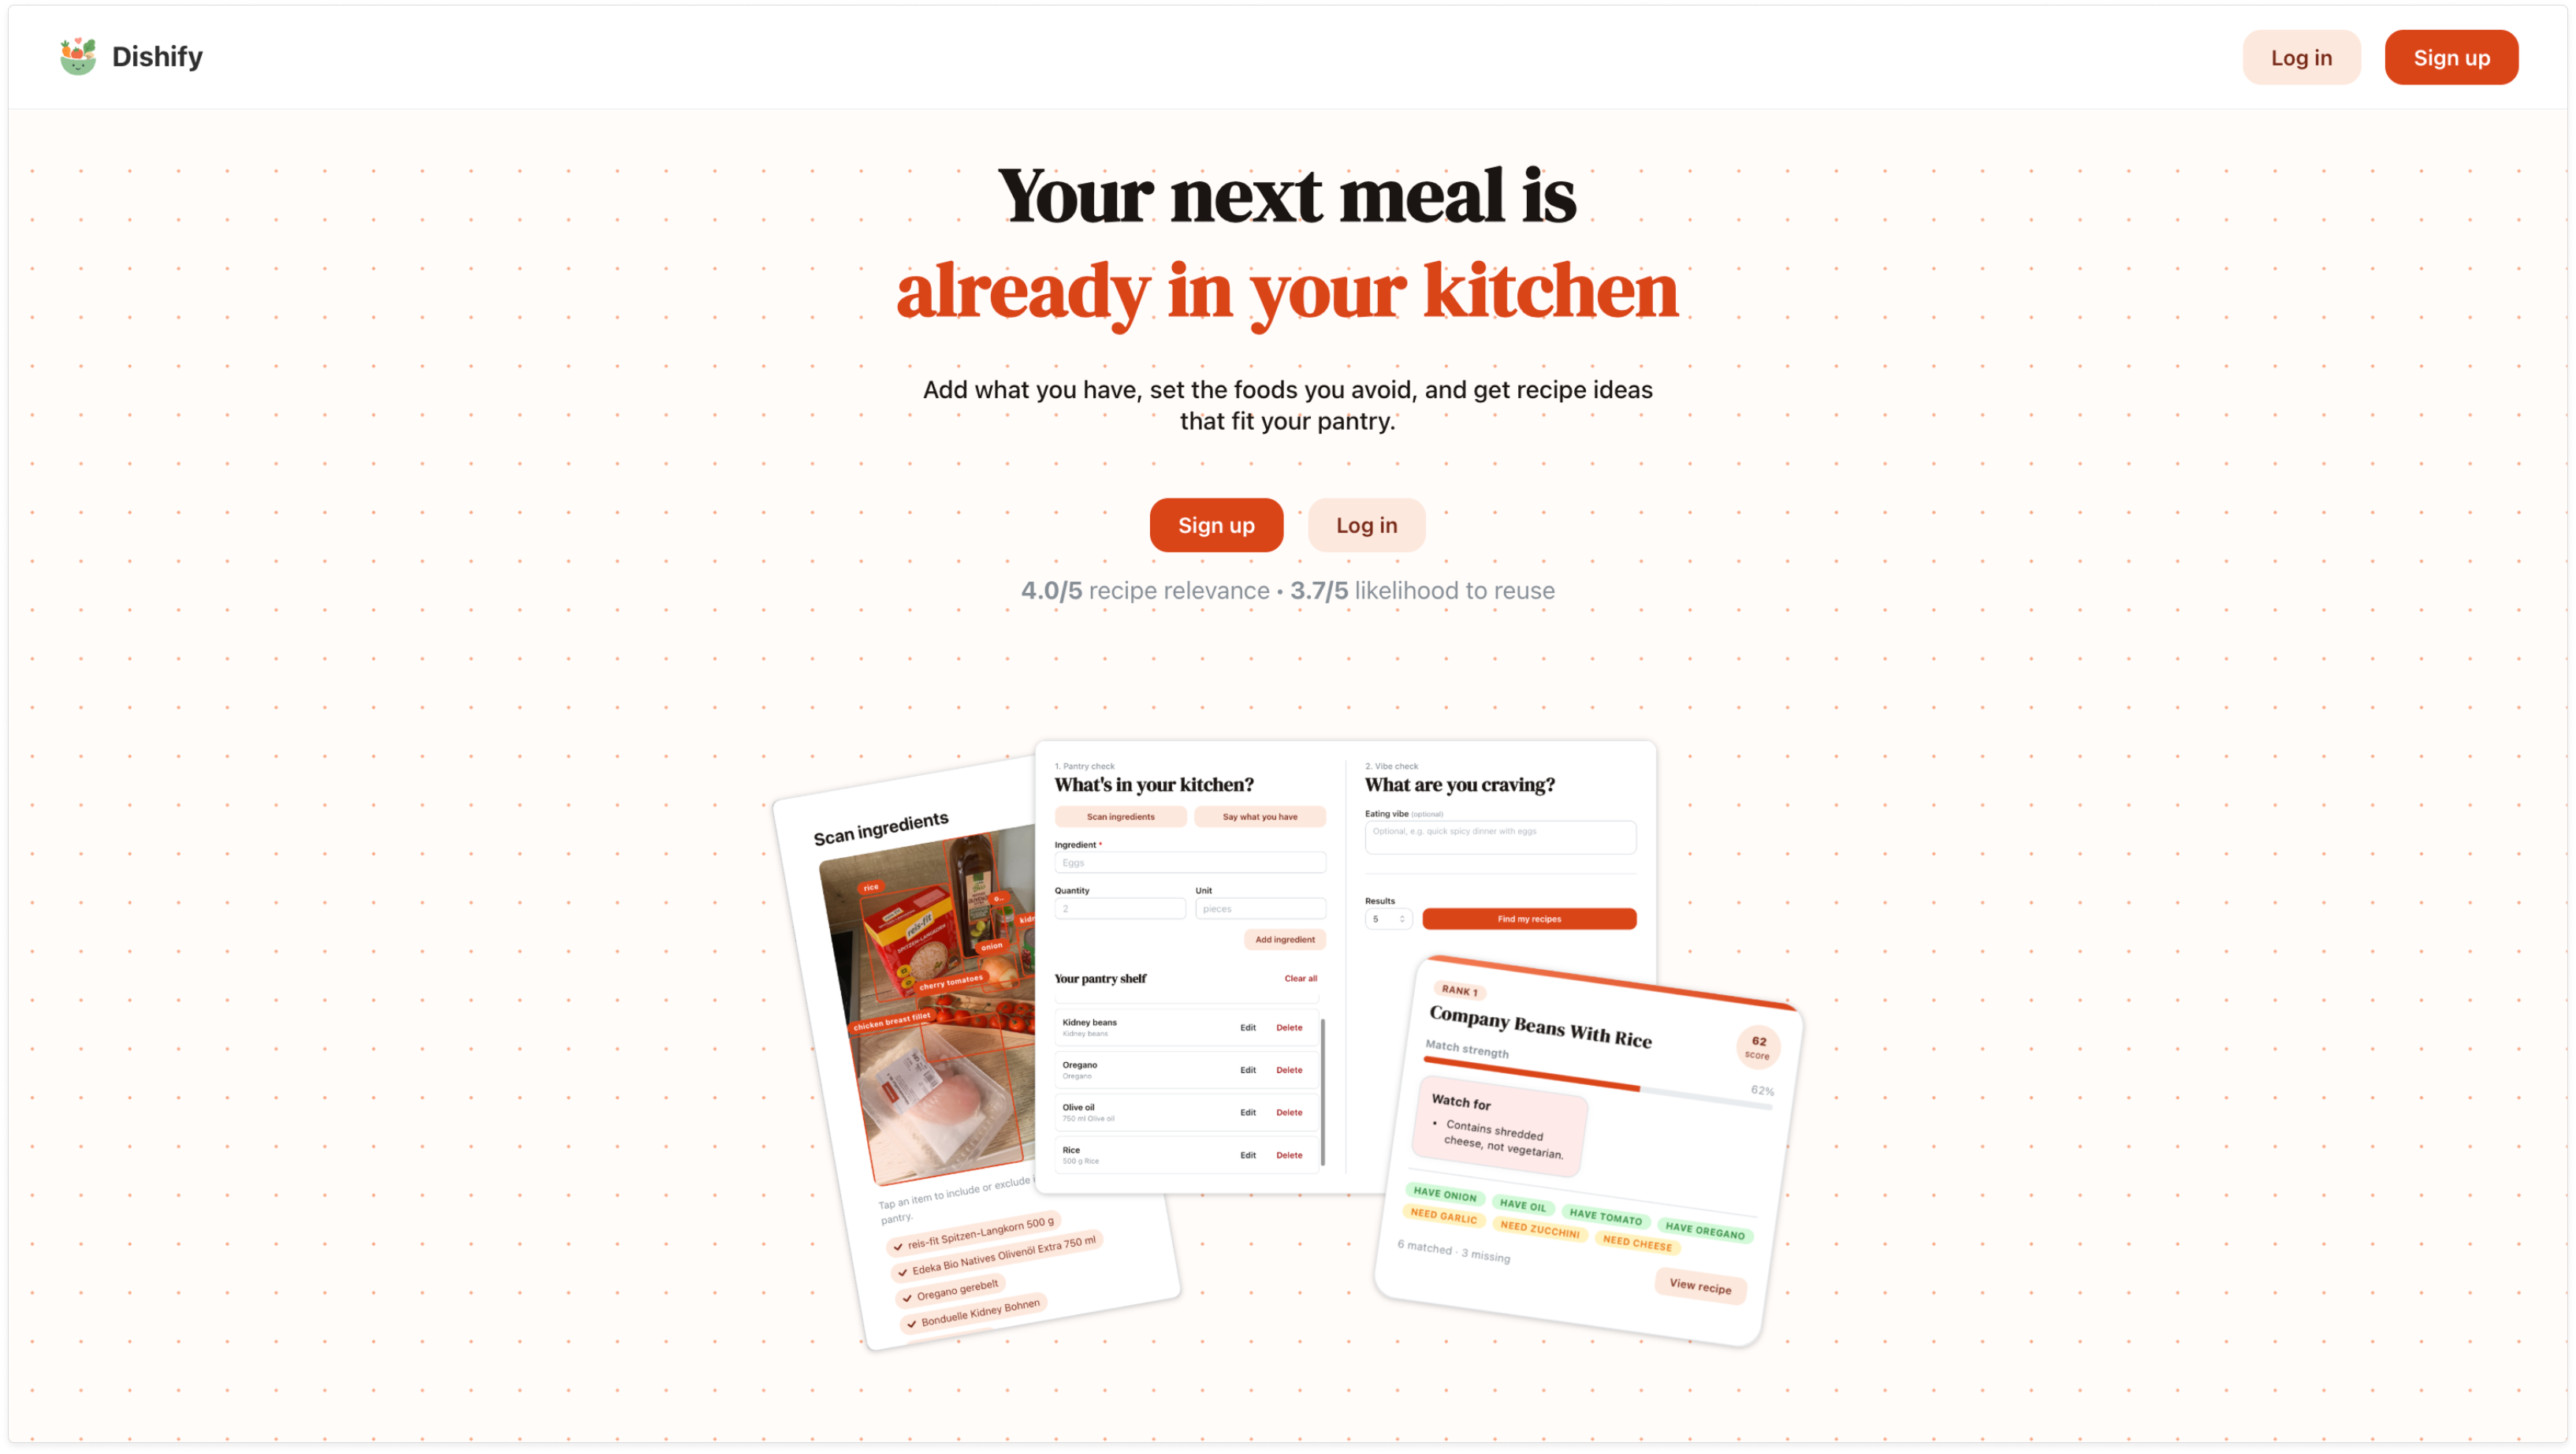
\includegraphics[width=\textwidth]{./Ressourcen/user-guide/landing-page.png}
    \captionof{figure}{The Dishify landing page.}
    \label{fig:ug-landing-page}
\end{center}

Dishify is available as an iOS app as well as on the web. Currently, only the web version is accessible. Find out more about Dishify here: \url{http://167.233.165.44}



\section{Features}

\subsection{Sign Up and Initial Preferences}
\begin{center}
    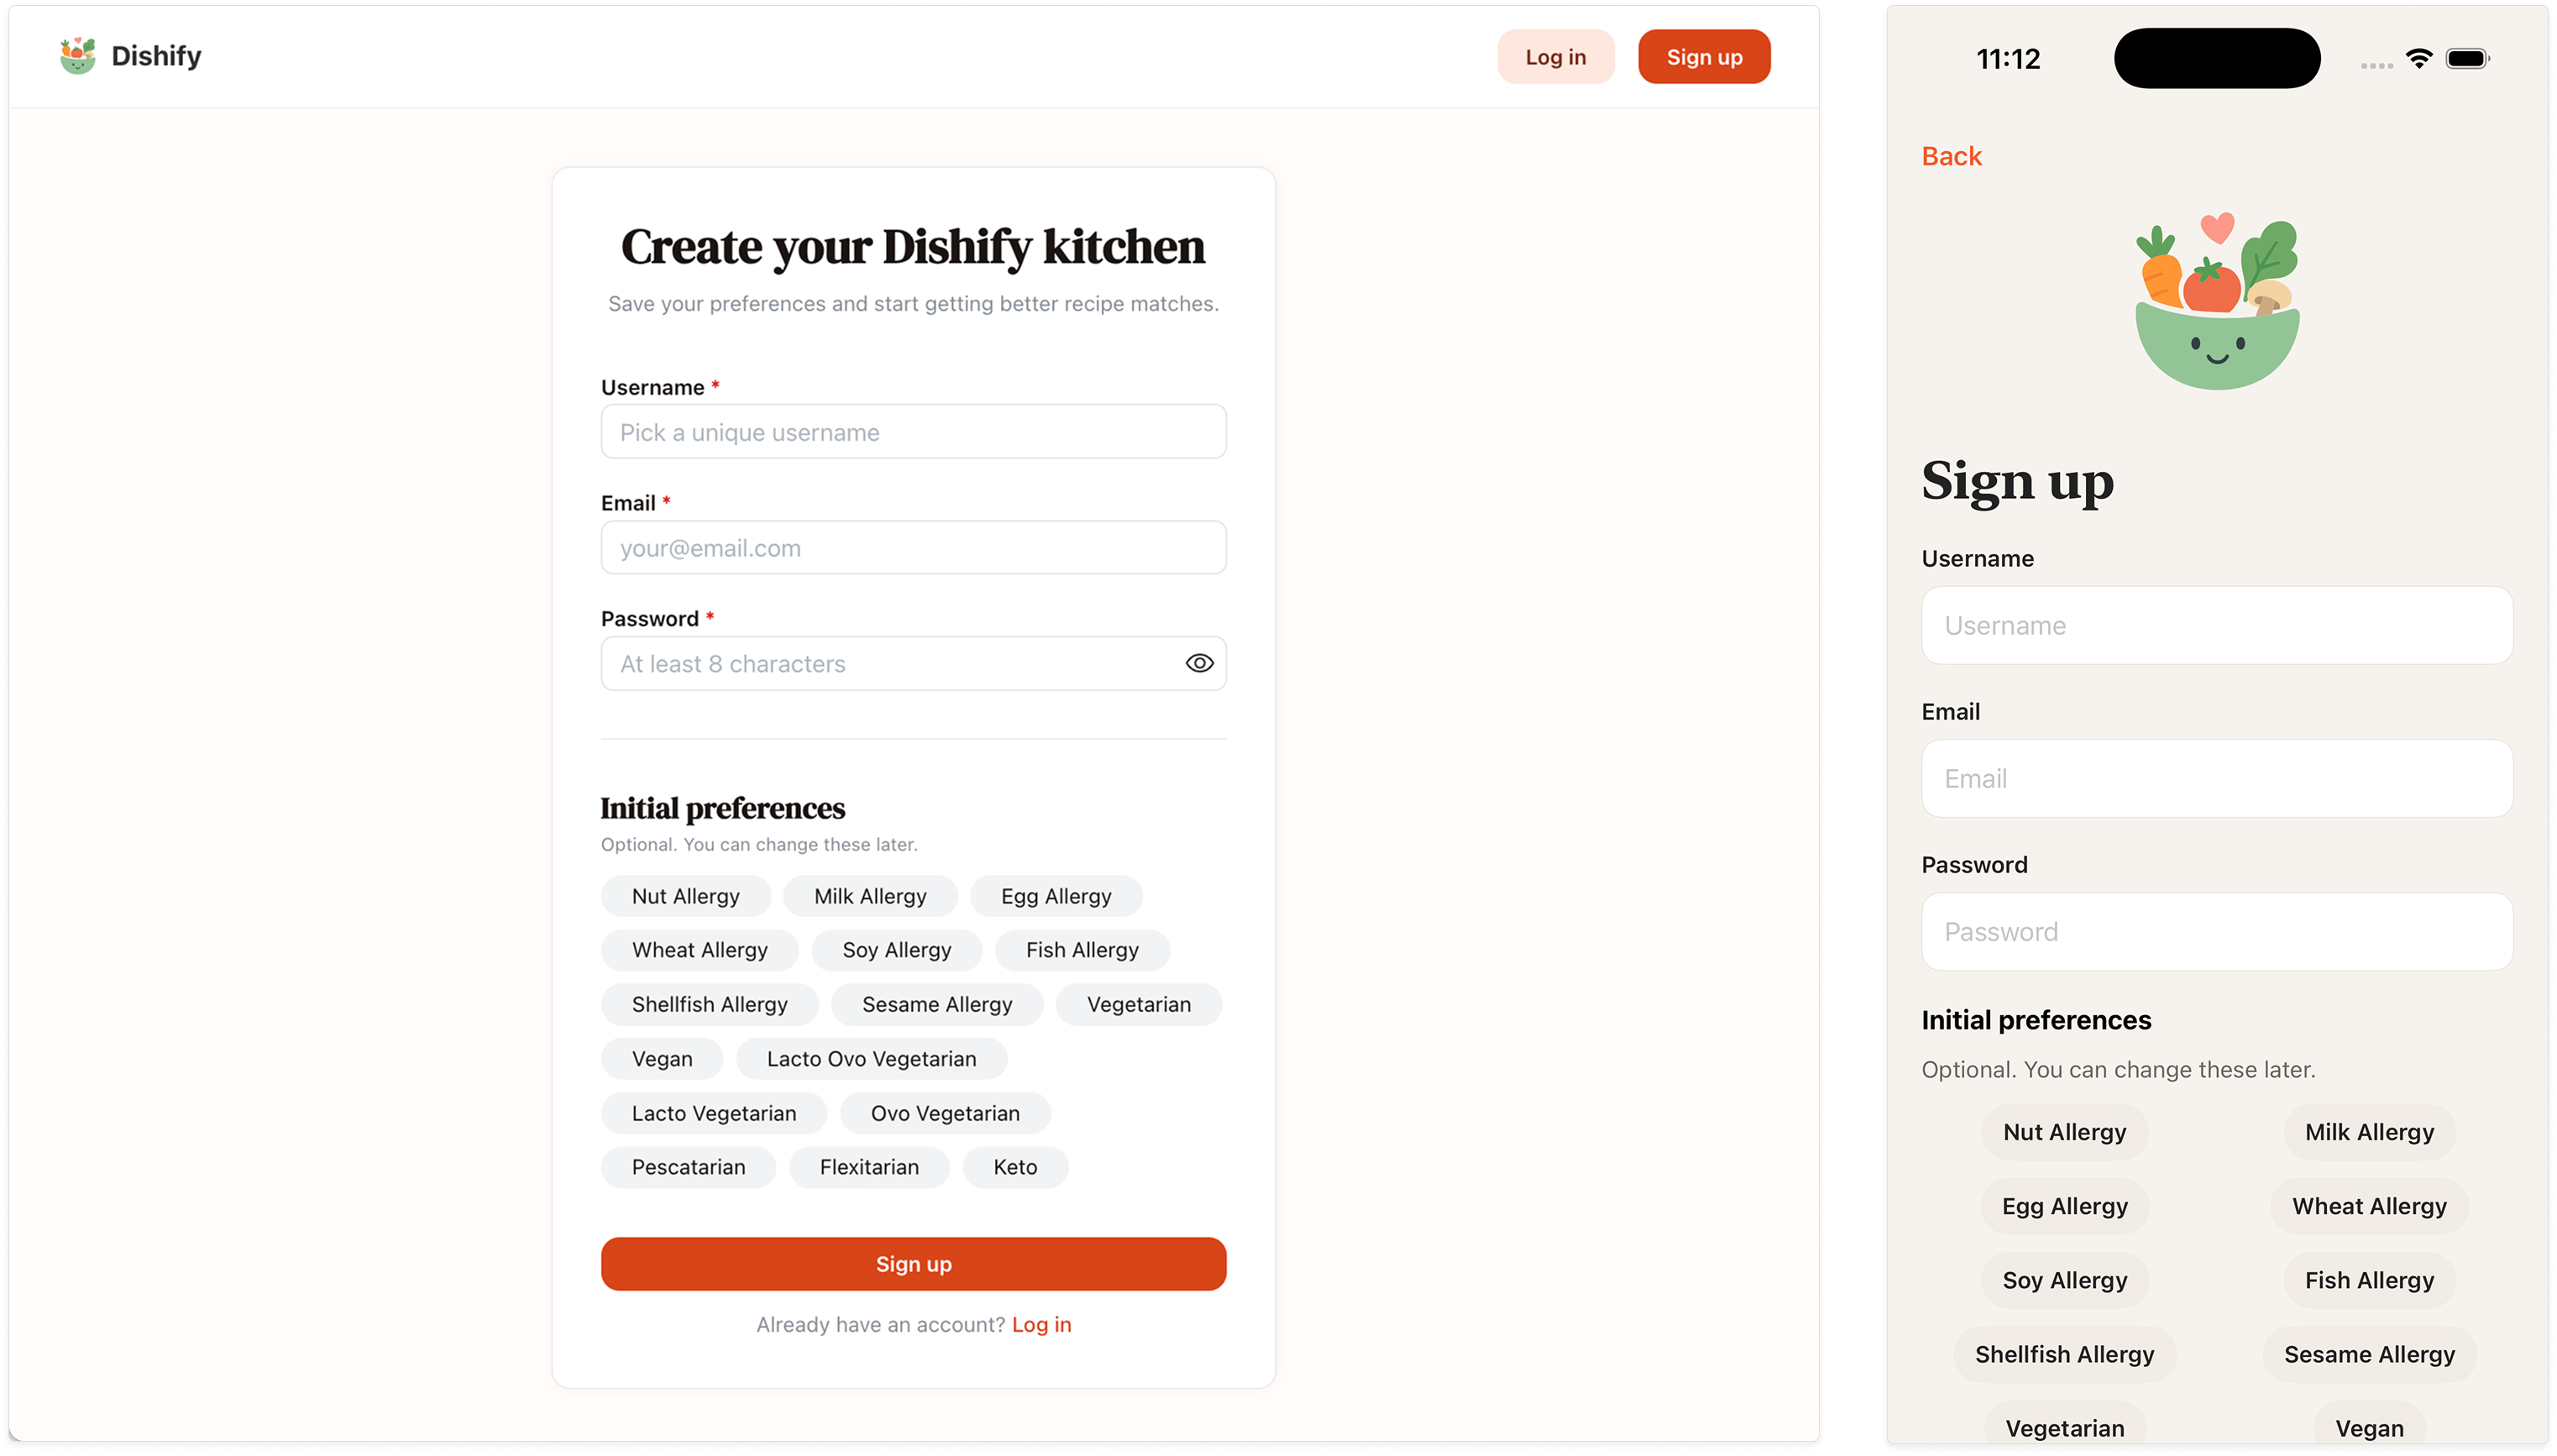
\includegraphics[width=\textwidth]{./Ressourcen/user-guide/signup-page.png}
    \captionof{figure}{The sign up page.}
    \label{fig:ug-signup}
\end{center}

During the sign up process, it is possible to specify preferences. The options include the most relevant preferences only. Additional options are available on the preferences page.



\subsection{Dietary, Allergy, and Restriction Filtering}
\begin{center}
    
\includegraphics[width=\textwidth]{./Ressourcen/user-guide/preferences.png}
    \captionof{figure}{The preferences page.}
    \label{fig:ug-preferences}
\end{center}
Dishify respects a plethora of preferences, including the categories allergies, diets, religious and ethical, medical and sensitivities, as well as ingredient exclusions.
Preferences can be changed at any time and Dishify will exclude respective recipes from its suggestions.



\subsection{Pantry-based Recipe Recommendation}
\begin{center}
    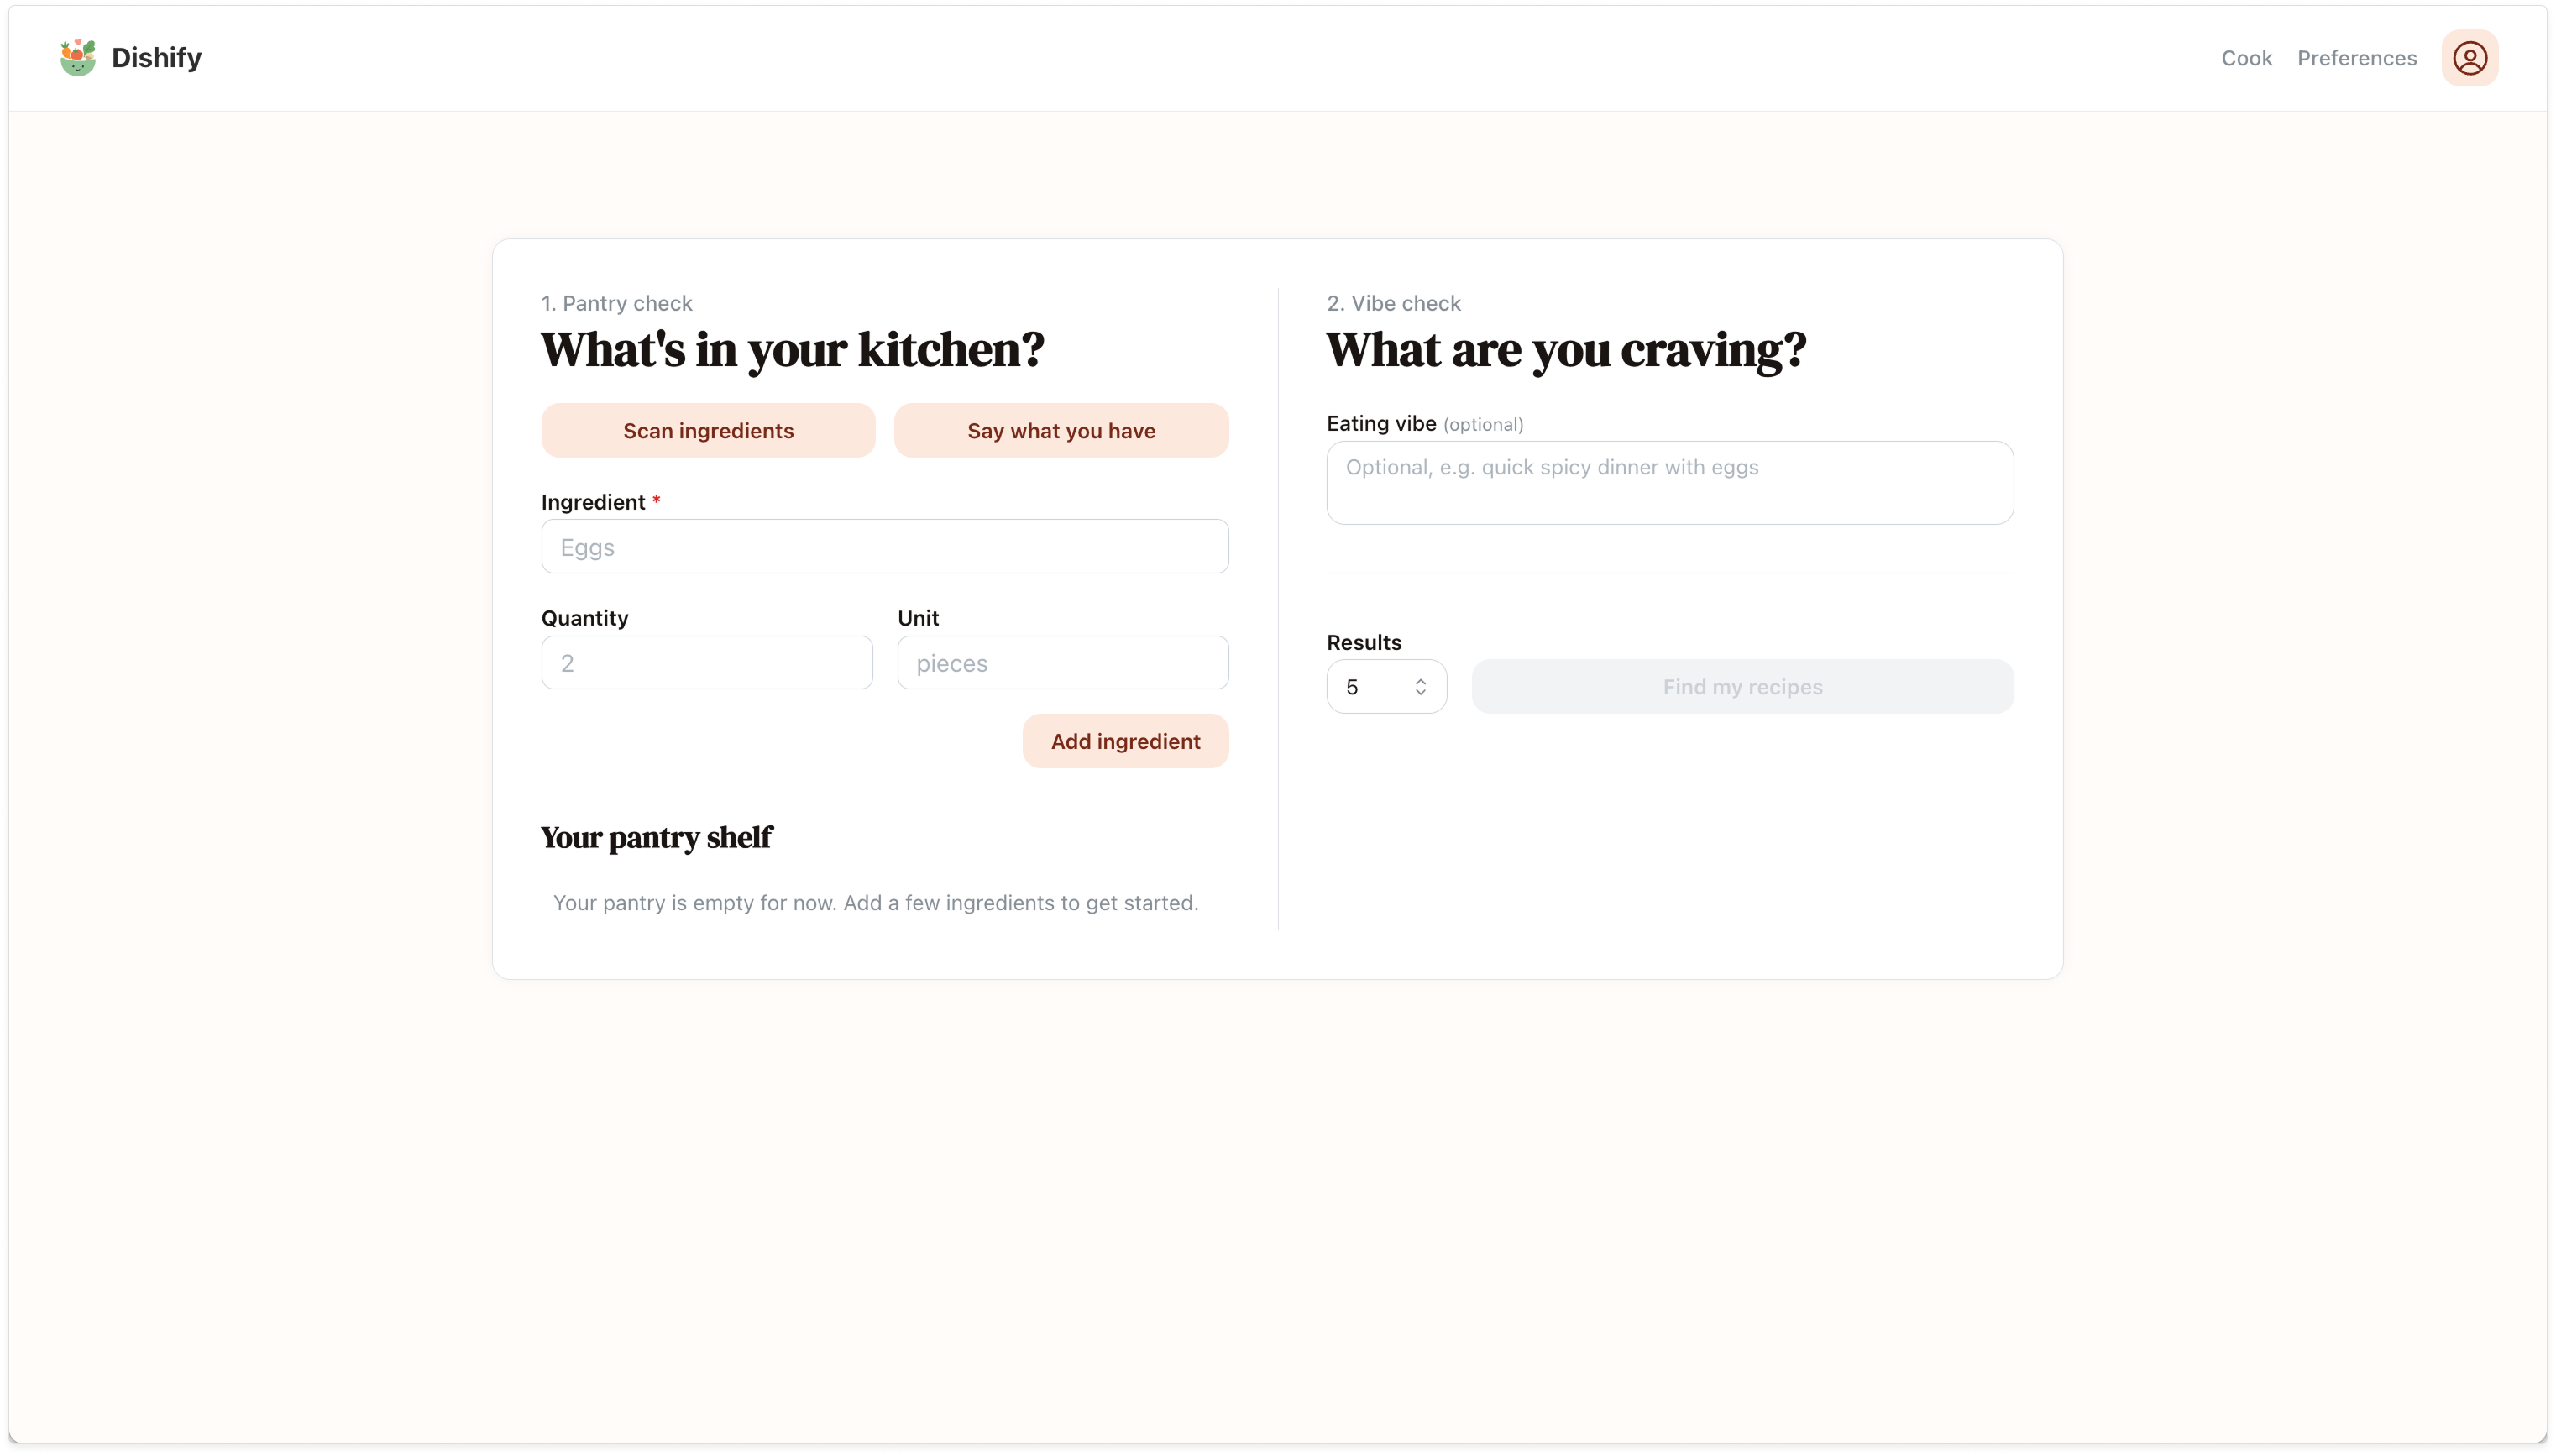
\includegraphics[width=\textwidth]{./Ressourcen/user-guide/ingredients.png}
    \captionof{figure}{The ingredients page.}
    \label{fig:ug-ingredients}
\end{center}
Dishify accepts ingredients as well as the eating vibe as input. Apart from the ingredient's name (e.g. eggs), the quantity (e.g. 2) as well as the unit of measure (e.g. pieces) can be specified.
The eating vibe (e.g. fast) provides the user with additional control over the recipe suggestions.

\begin{center}
    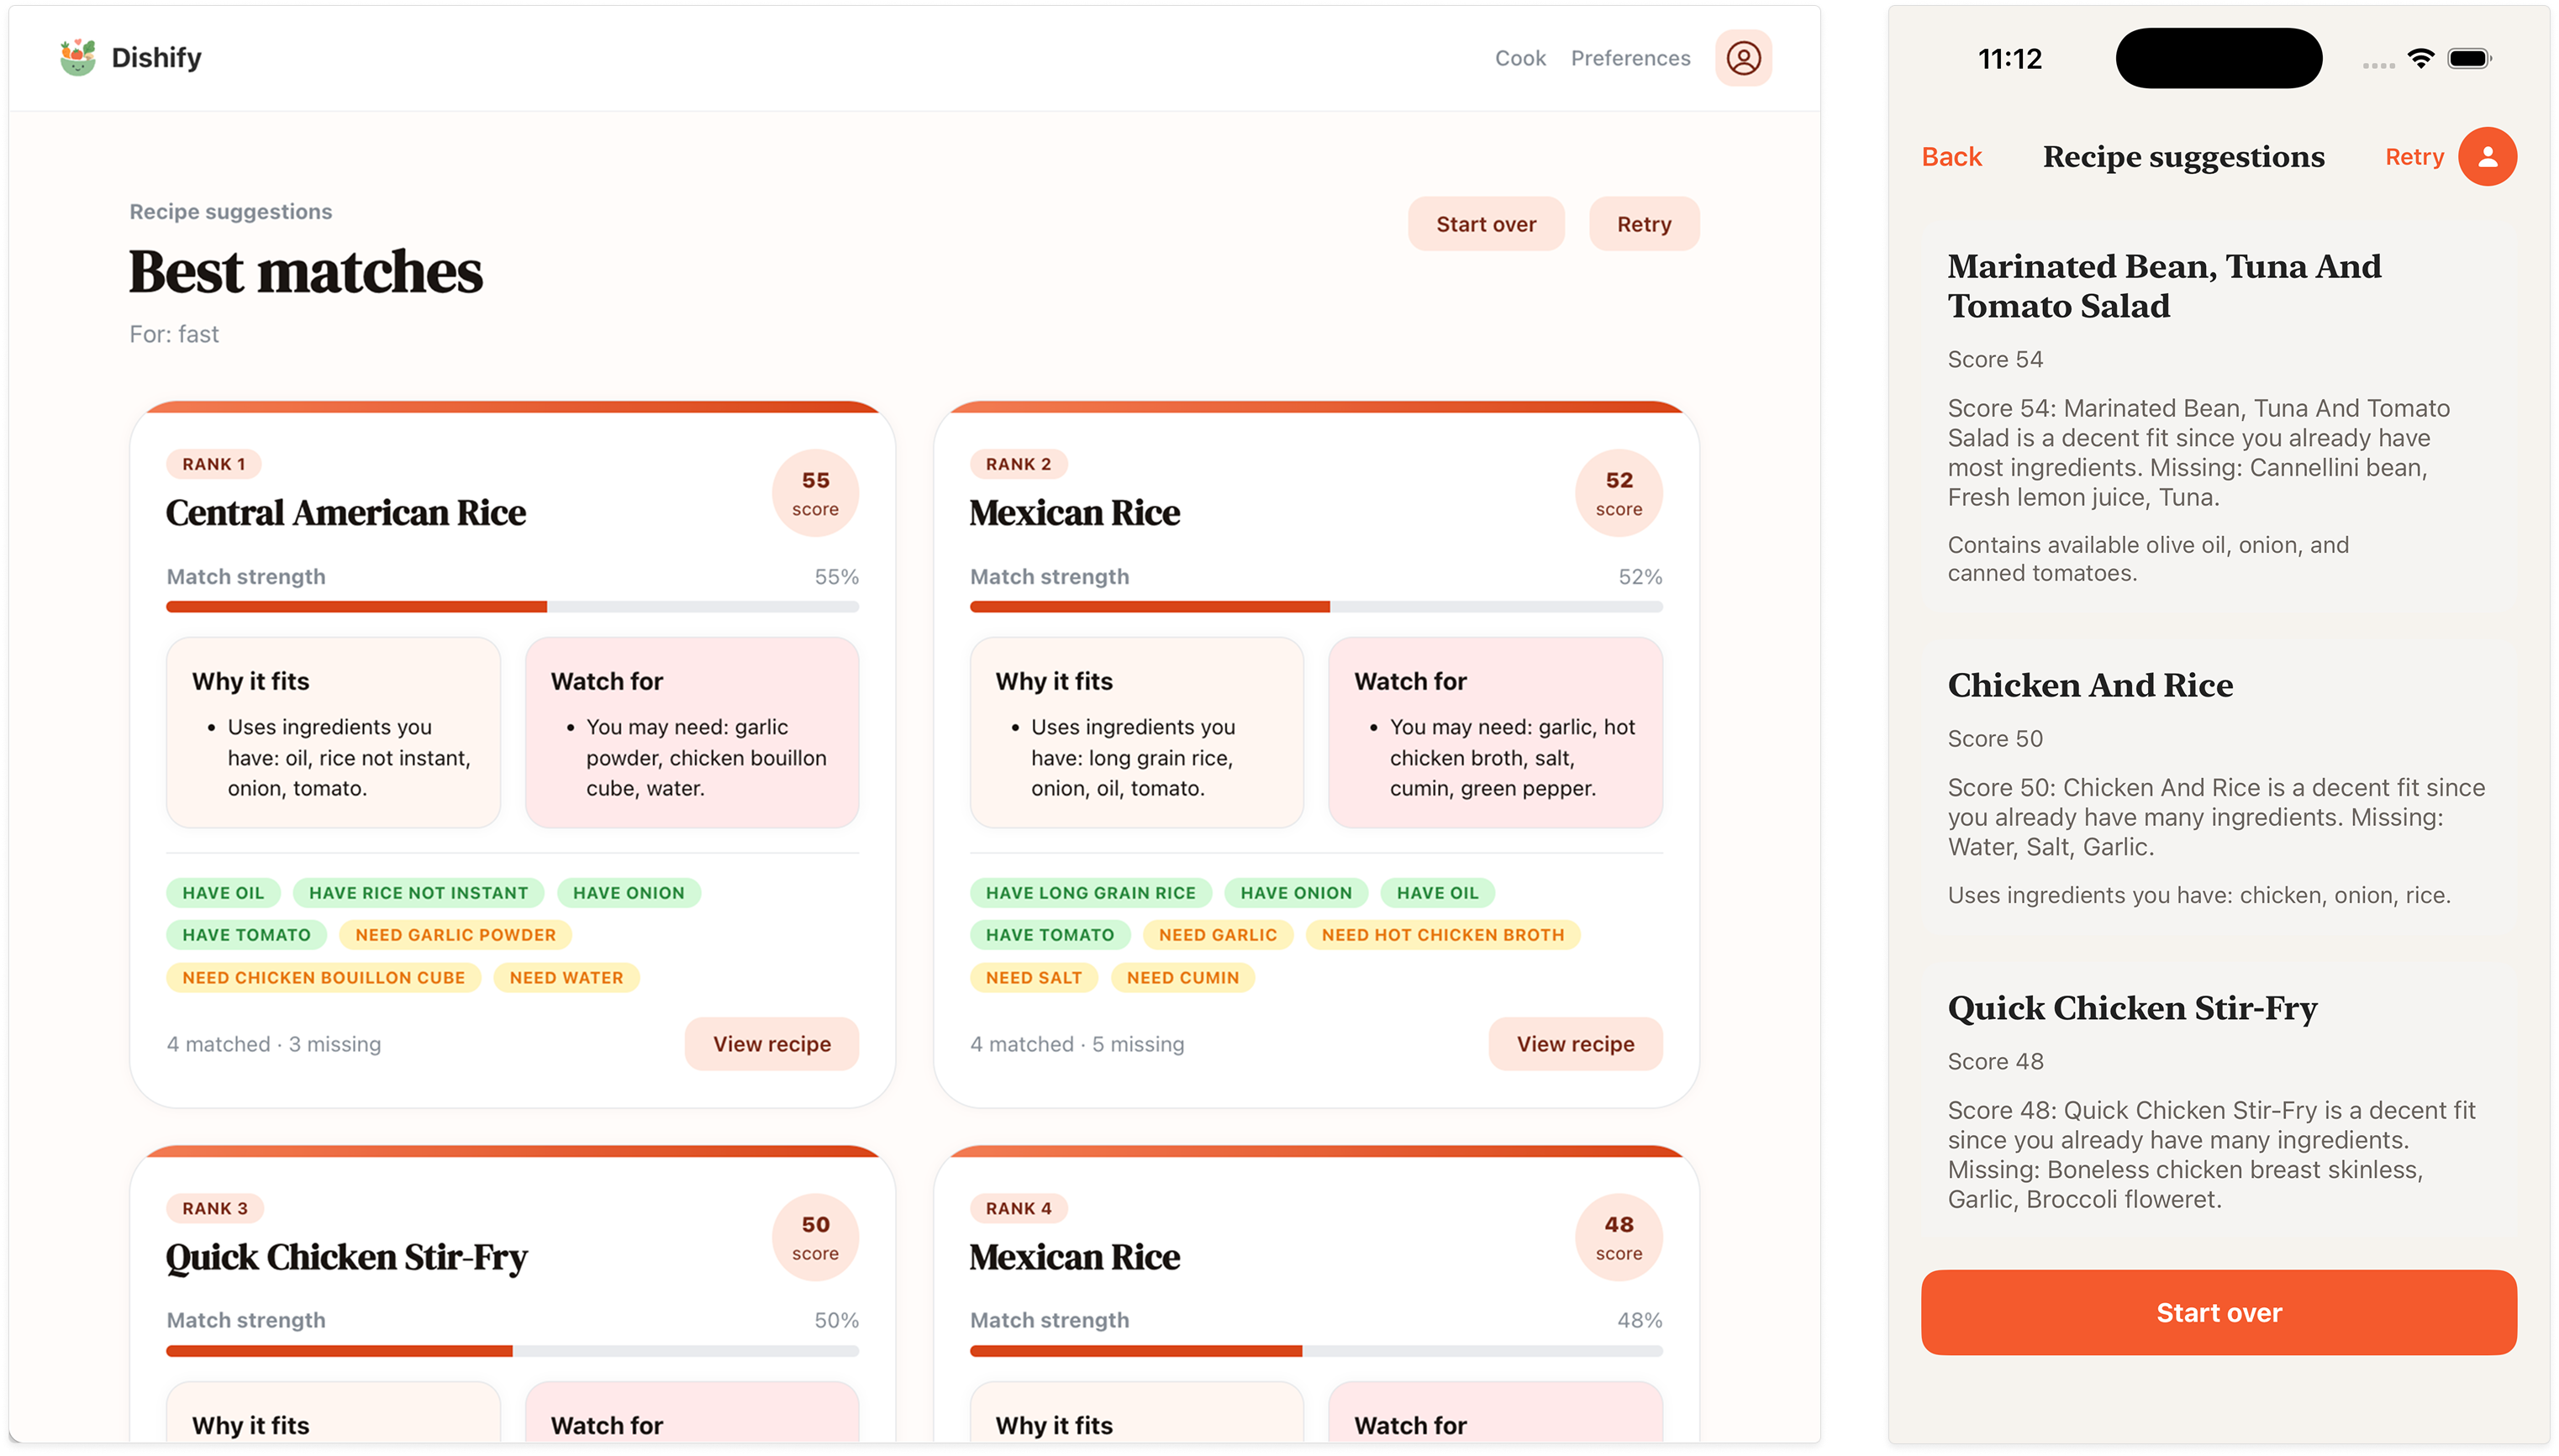
\includegraphics[width=\textwidth]{./Ressourcen/user-guide/results.png}
    \captionof{figure}{The results page.}
    \label{fig:ug-results}
\end{center}
The suggested recipes are ordered by a relevance score – a metric that shows how well a recipe fits the search and pantry: a mix of how closely it matches what you're looking for, and how many ingredients you already have on hand. 
For each suggestion Dishify displays the number of missing respectively available ingredients. Some of these ingredients are visible at a glance.



\subsection{Voice Input}
\begin{center}
    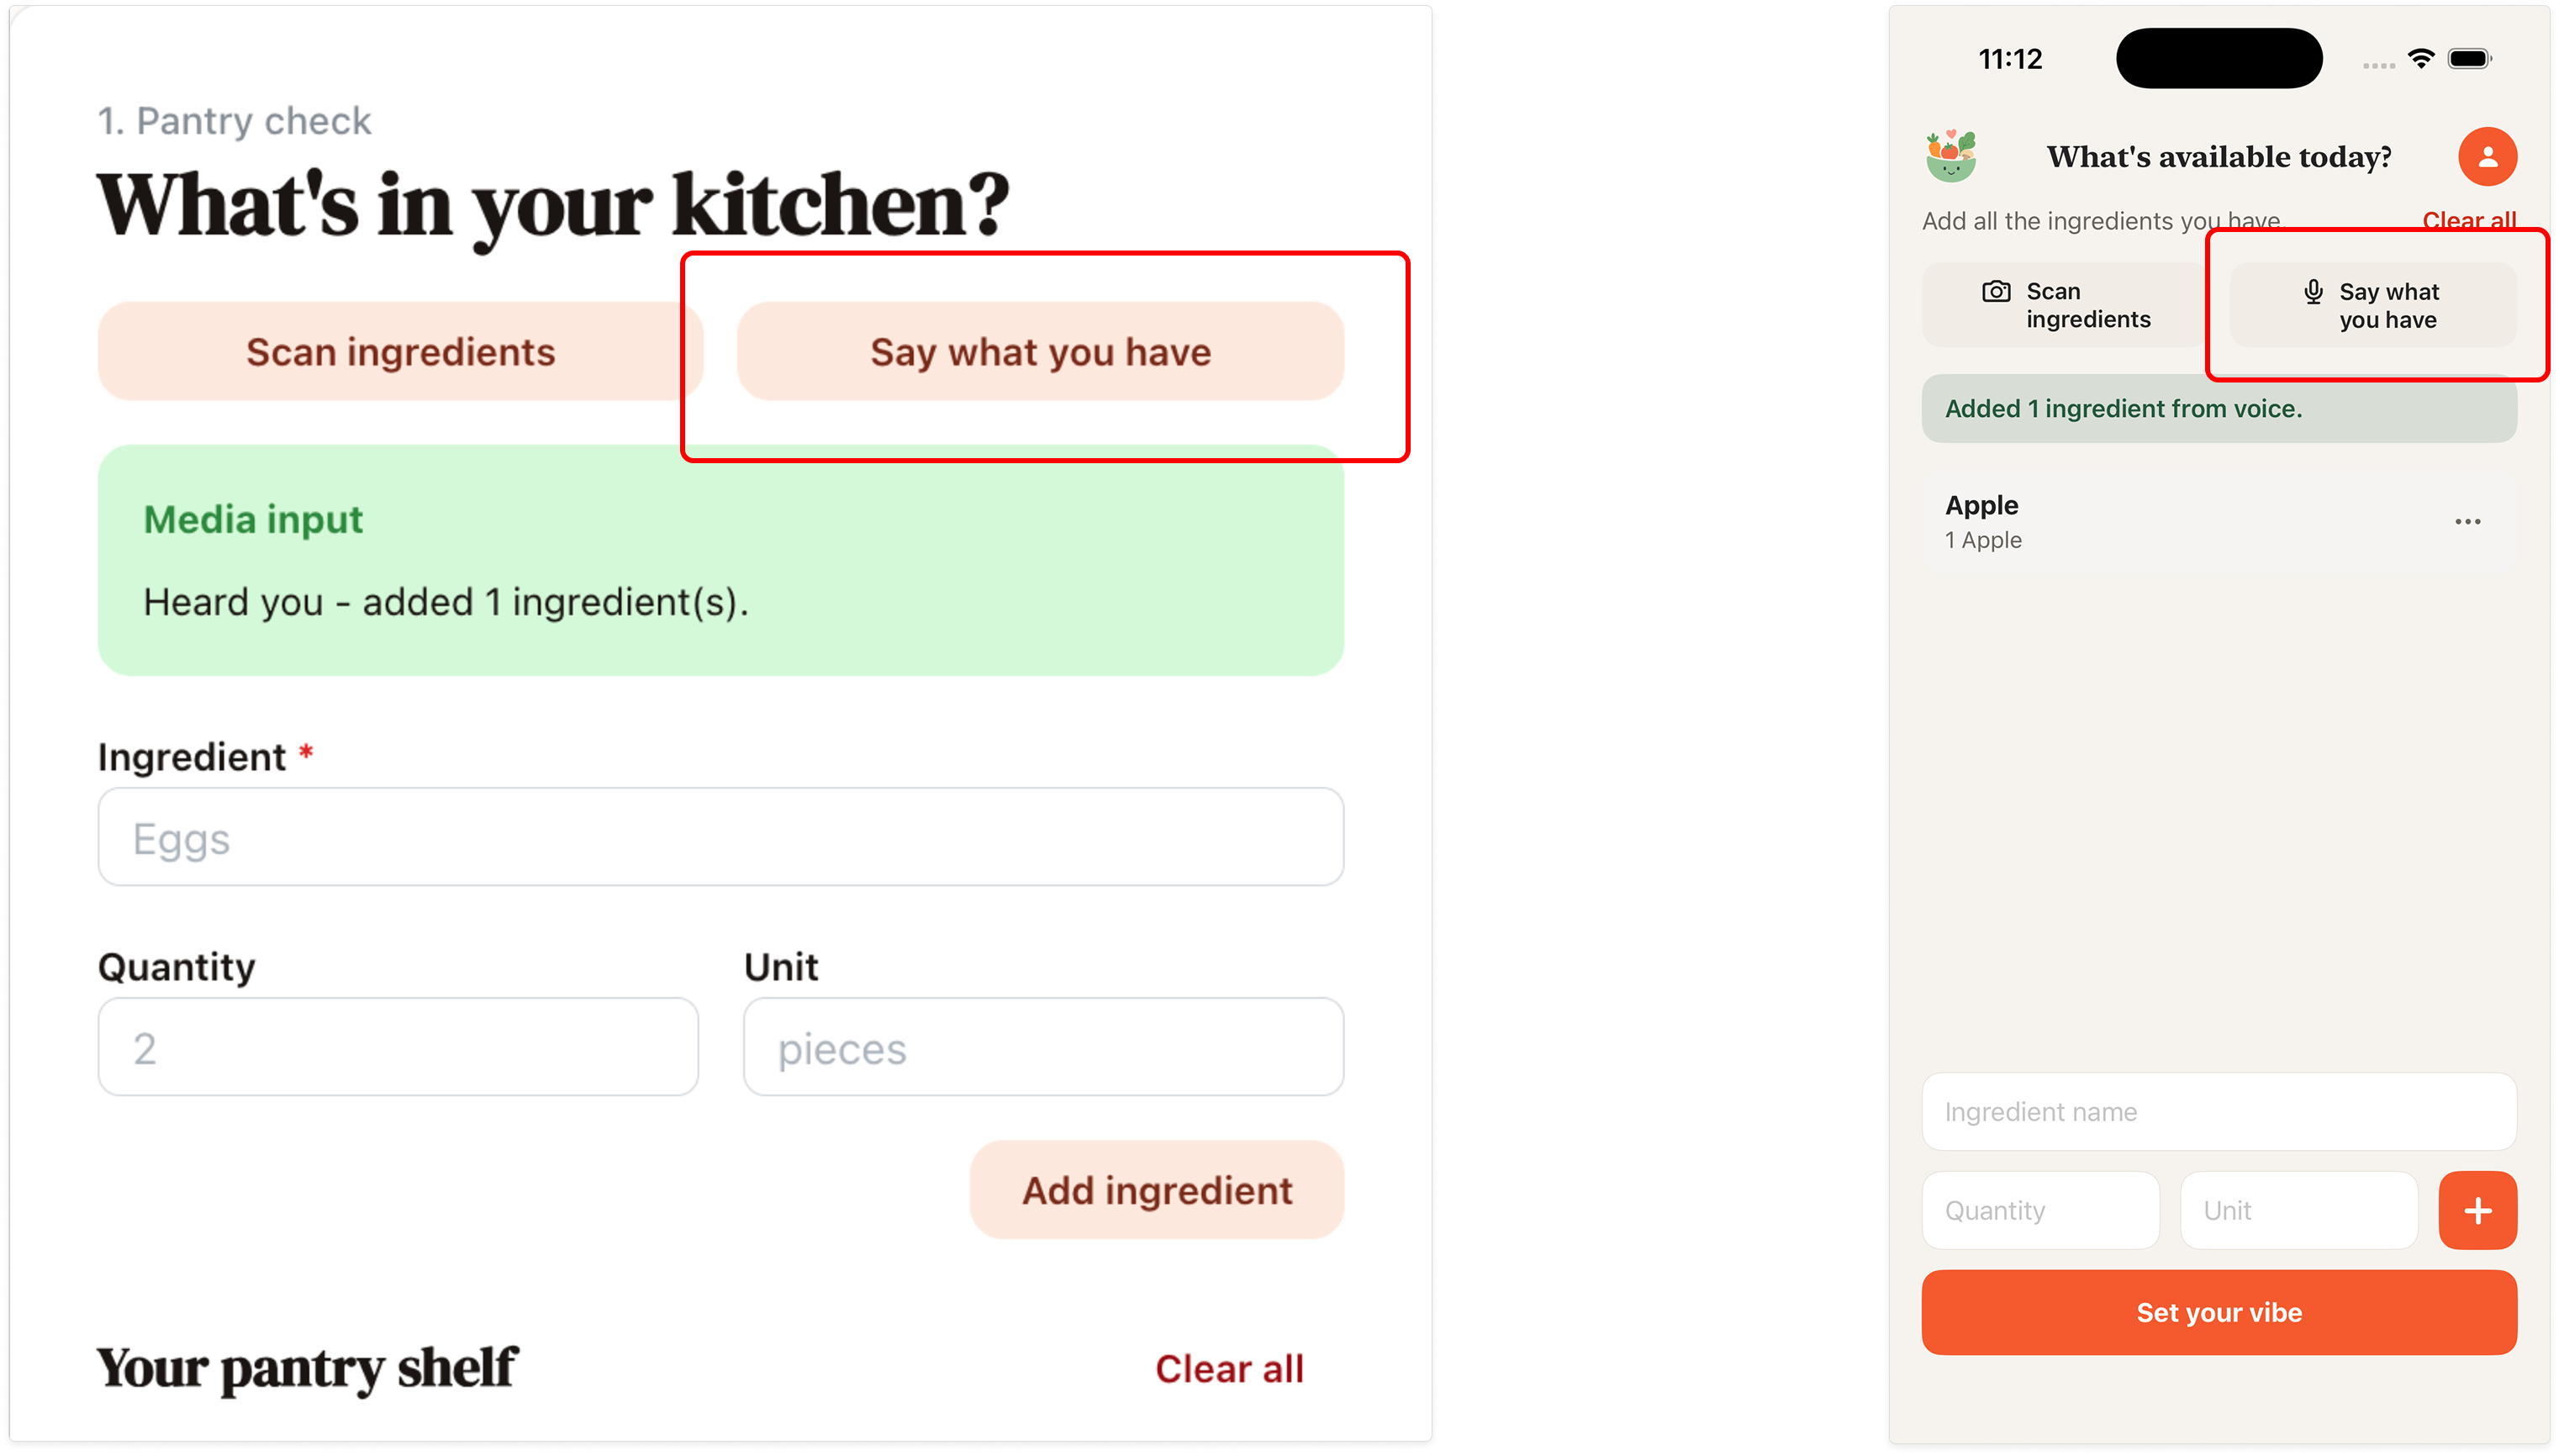
\includegraphics[width=\textwidth]{./Ressourcen/user-guide/voice.png}
    \captionof{figure}{Dishify understands voice input.}
    \label{fig:ug-voice}
\end{center}
Apart from text input Dishify understands voice input. Say what you have and Dishify adds it to the pantry shelf. 



\subsection{Image-based Ingredient Detection}
\begin{center}
    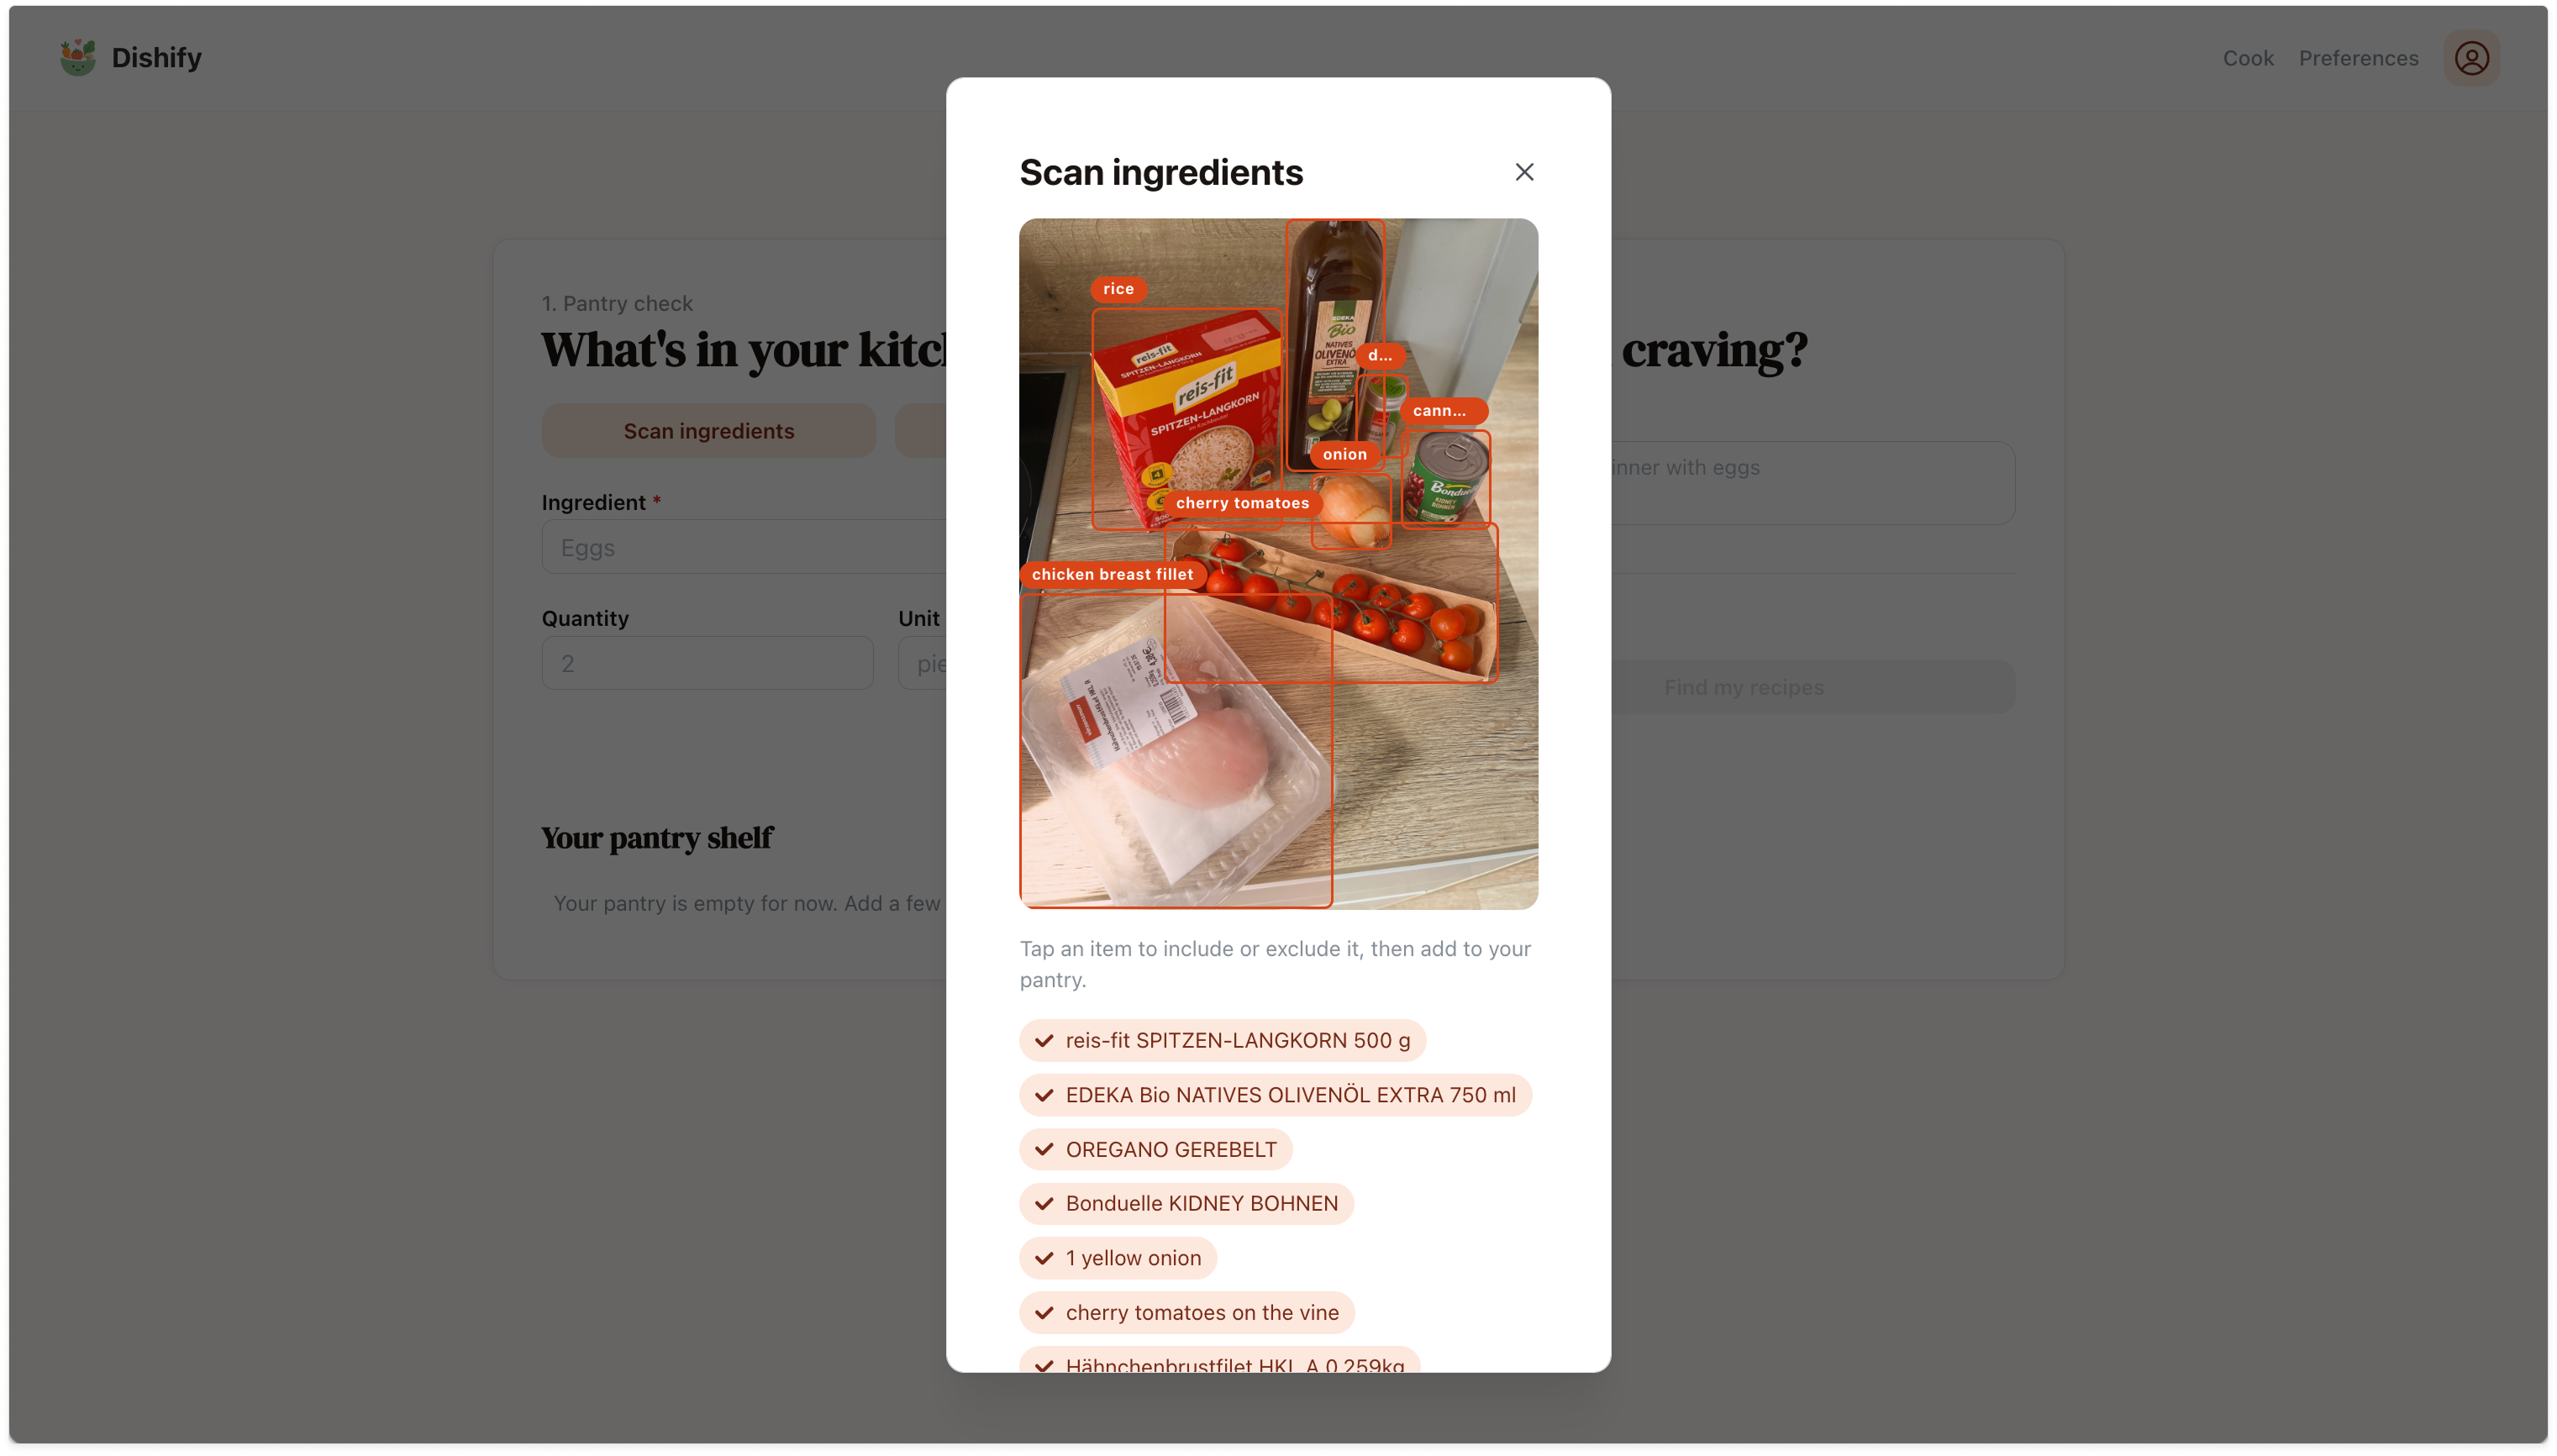
\includegraphics[width=\textwidth]{./Ressourcen/user-guide/image.png}
    \captionof{figure}{Dishify understands image input.}
    \label{fig:ug-image}
\end{center}
Dishify also allows for ingredient input via images (camera or image upload). Recognized ingredients are framed by boxes and ingredients can be deselected individually. 


\subsection{Recipe Detail}
\begin{center}
    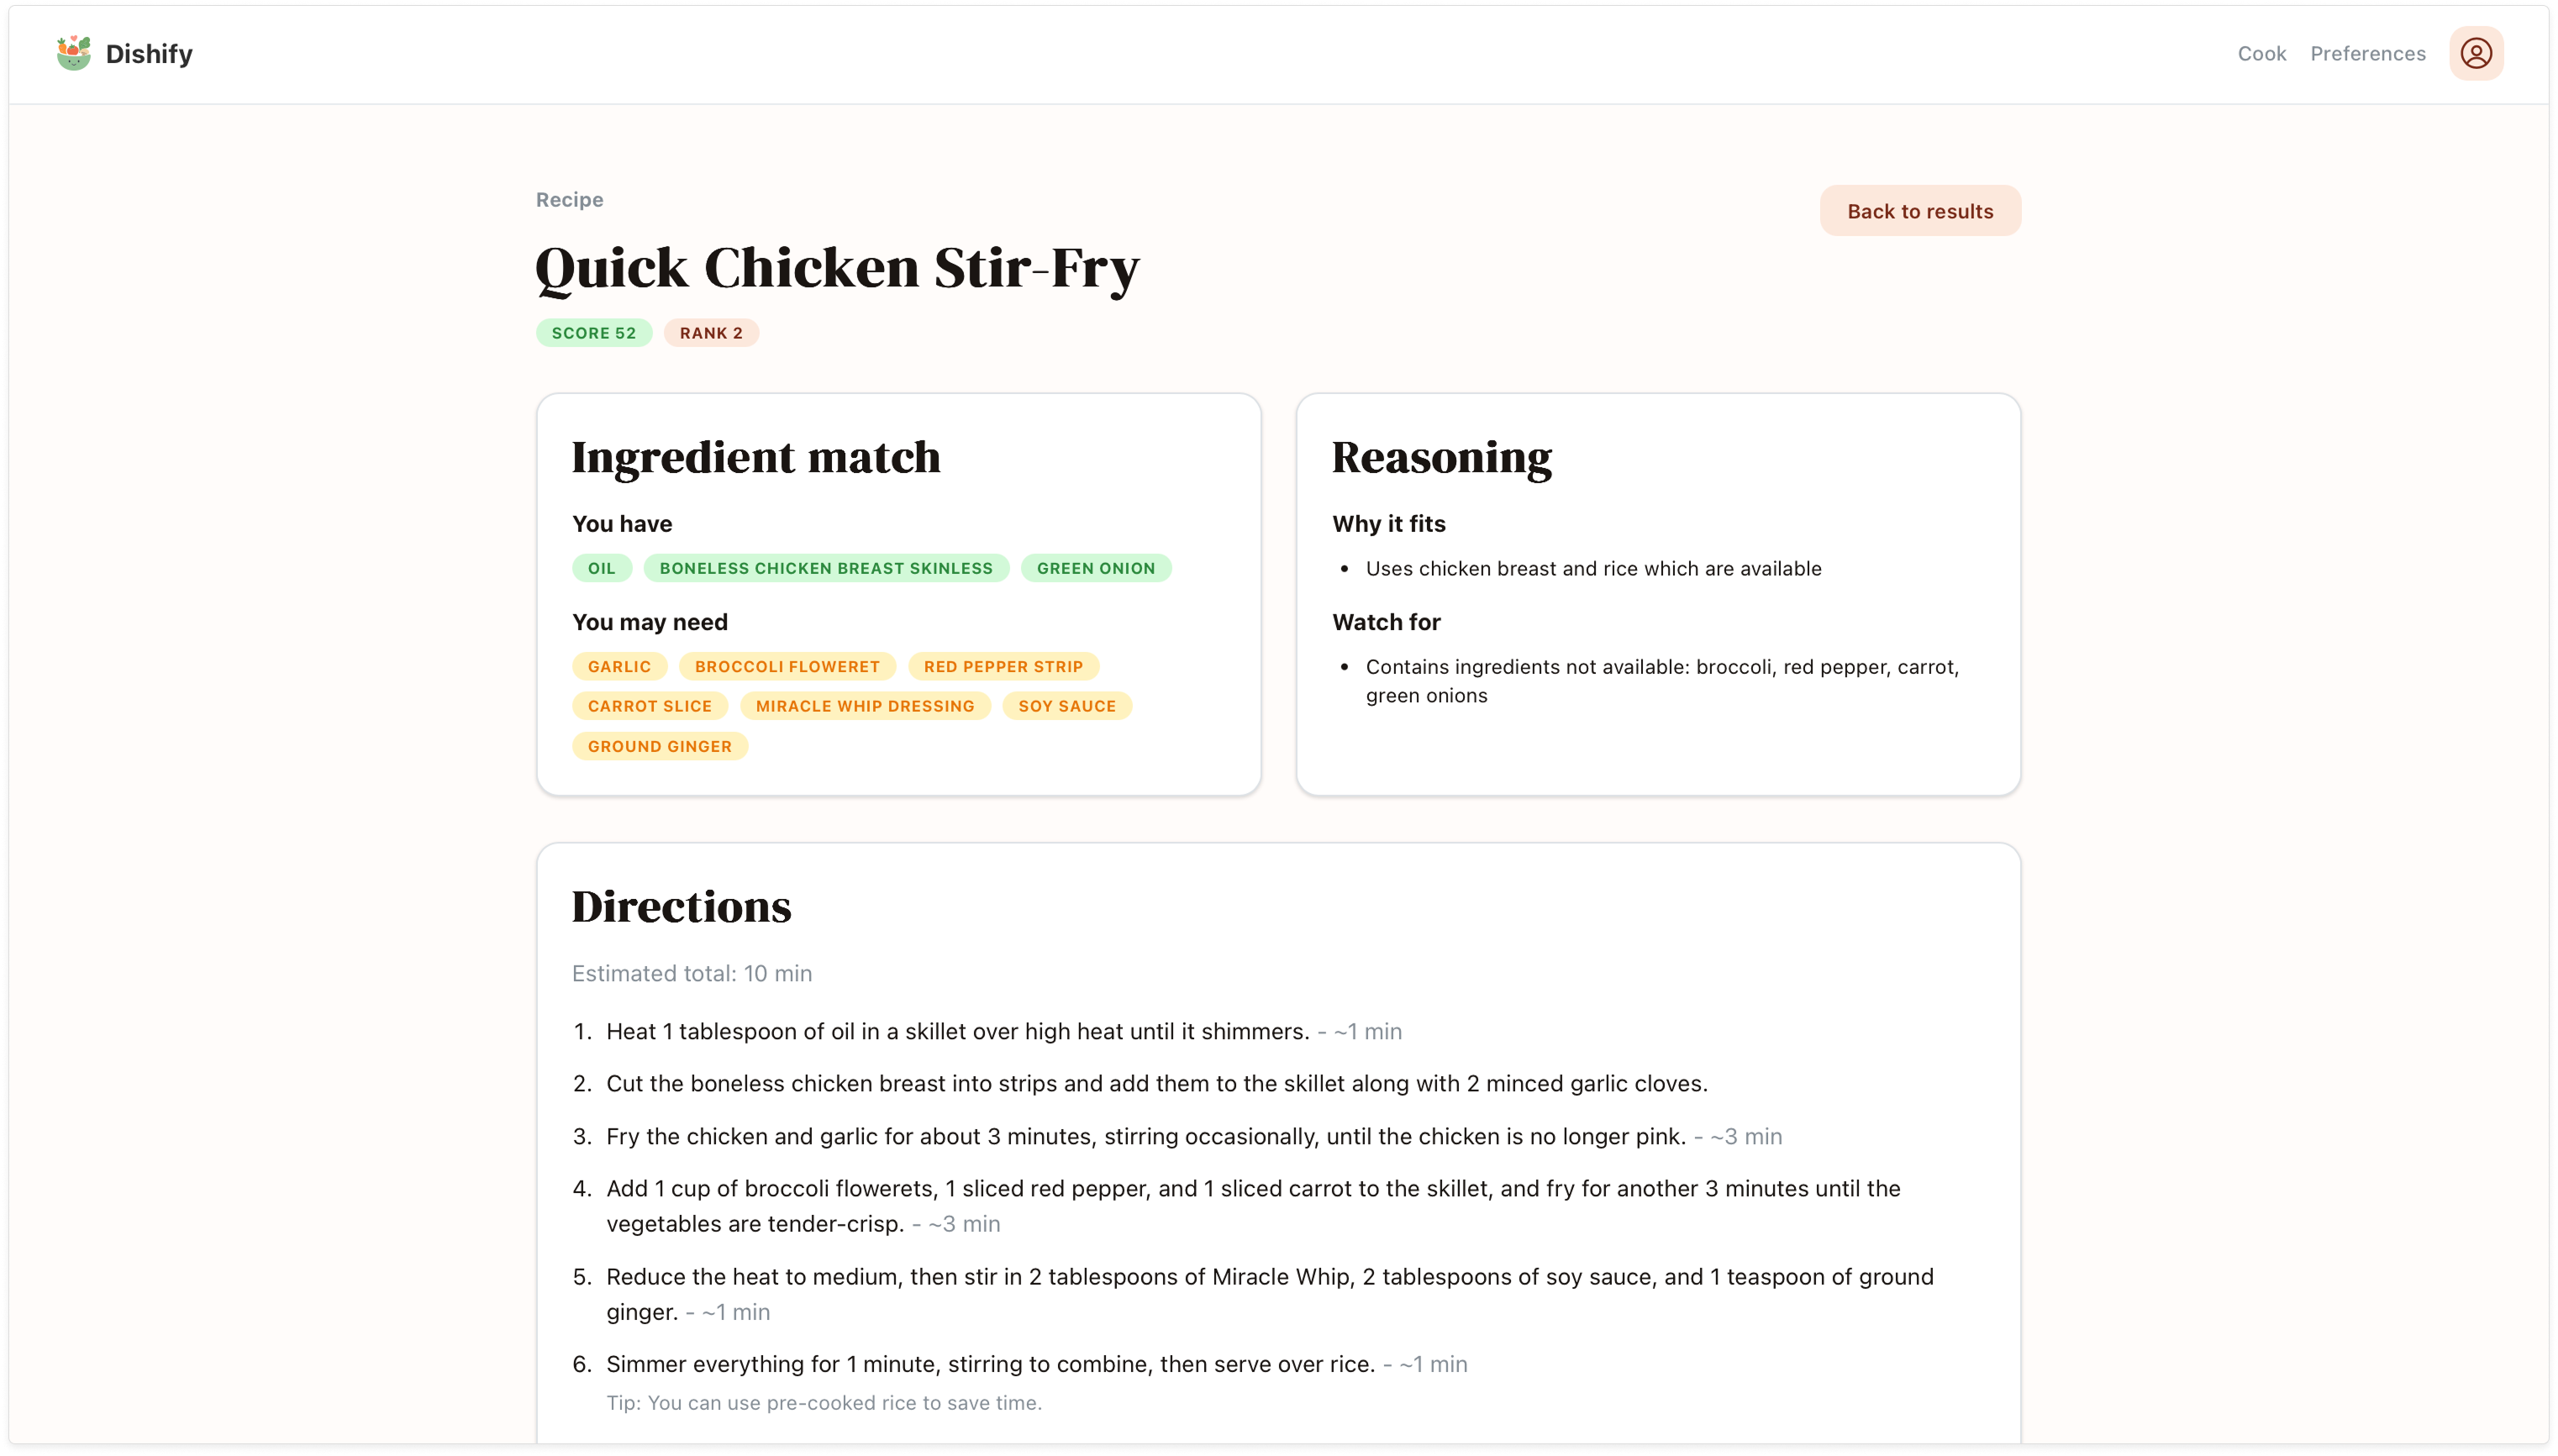
\includegraphics[width=\textwidth]{./Ressourcen/user-guide/recipe.png}
    \captionof{figure}{The recipe page.}
    \label{fig:ug-recipe}
\end{center}
The recipe page lists missing and available ingredients, an explanation why Dishify suggested the recipe, lists things to watch out for, and the steps to prepare the recipe. 

% !TeX root = ../CourseReport.tex
%=============================================================================
%  PART 2 --- PROJECT MANAGEMENT REPORT
%  PAGE BUDGET: 8 pages (excluding title, ToC)          Rubric weight: 20 pts
%
%  Required sections (all expected by the grading criteria):
%    - Overall Project Vision (scope, key deliverables, boundaries)
%    - Project Timeline (stand-alone Gantt chart, categories, subtasks, owners)
%    - System Architecture (structure + main components)
%    - Method (methodologies; MUST include a Prompt Engineering subsection)
%    - Team Chart (members, roles, contributions)
%    - Current Progress and Future Plans
%    - Pitch Video (~60s) -- submitted as an attachment; link it here
%=============================================================================
\chapter{Project Management Report}
\label{ch:project-management}

\section{Overall Project Vision}
% TODO: Project scope, key deliverables, and explicit boundaries (what is out of
% scope). State the problem and the target outcome.

\section{Project Timeline}
% TODO: Insert a STAND-ALONE Gantt chart (readable without the surrounding text).
% Cluster work into categories (feature/team categories); show key subtasks only
% (not every task); make crew/person responsibilities clear.
% Options: pgfgantt package, or export an image and \includegraphics it.
\begin{figure}[!ht]
    \centering
    \fbox{\rule{0pt}{55mm}\rule{130mm}{0pt}}%
    % \includegraphics[width=\textwidth]{./Ressourcen/gantt.png}
    \caption{Project timeline and milestones (Gantt chart).}
    \label{fig:pm-gantt}
\end{figure}

\section{System Architecture}
% TODO: Technical details of the system structure and main components
% (gateway, recommendation, retrieval, reasoning, ingest, indexing, user;
% Qdrant, Keycloak; web + iOS clients).
\begin{figure}[!ht]
    \centering
    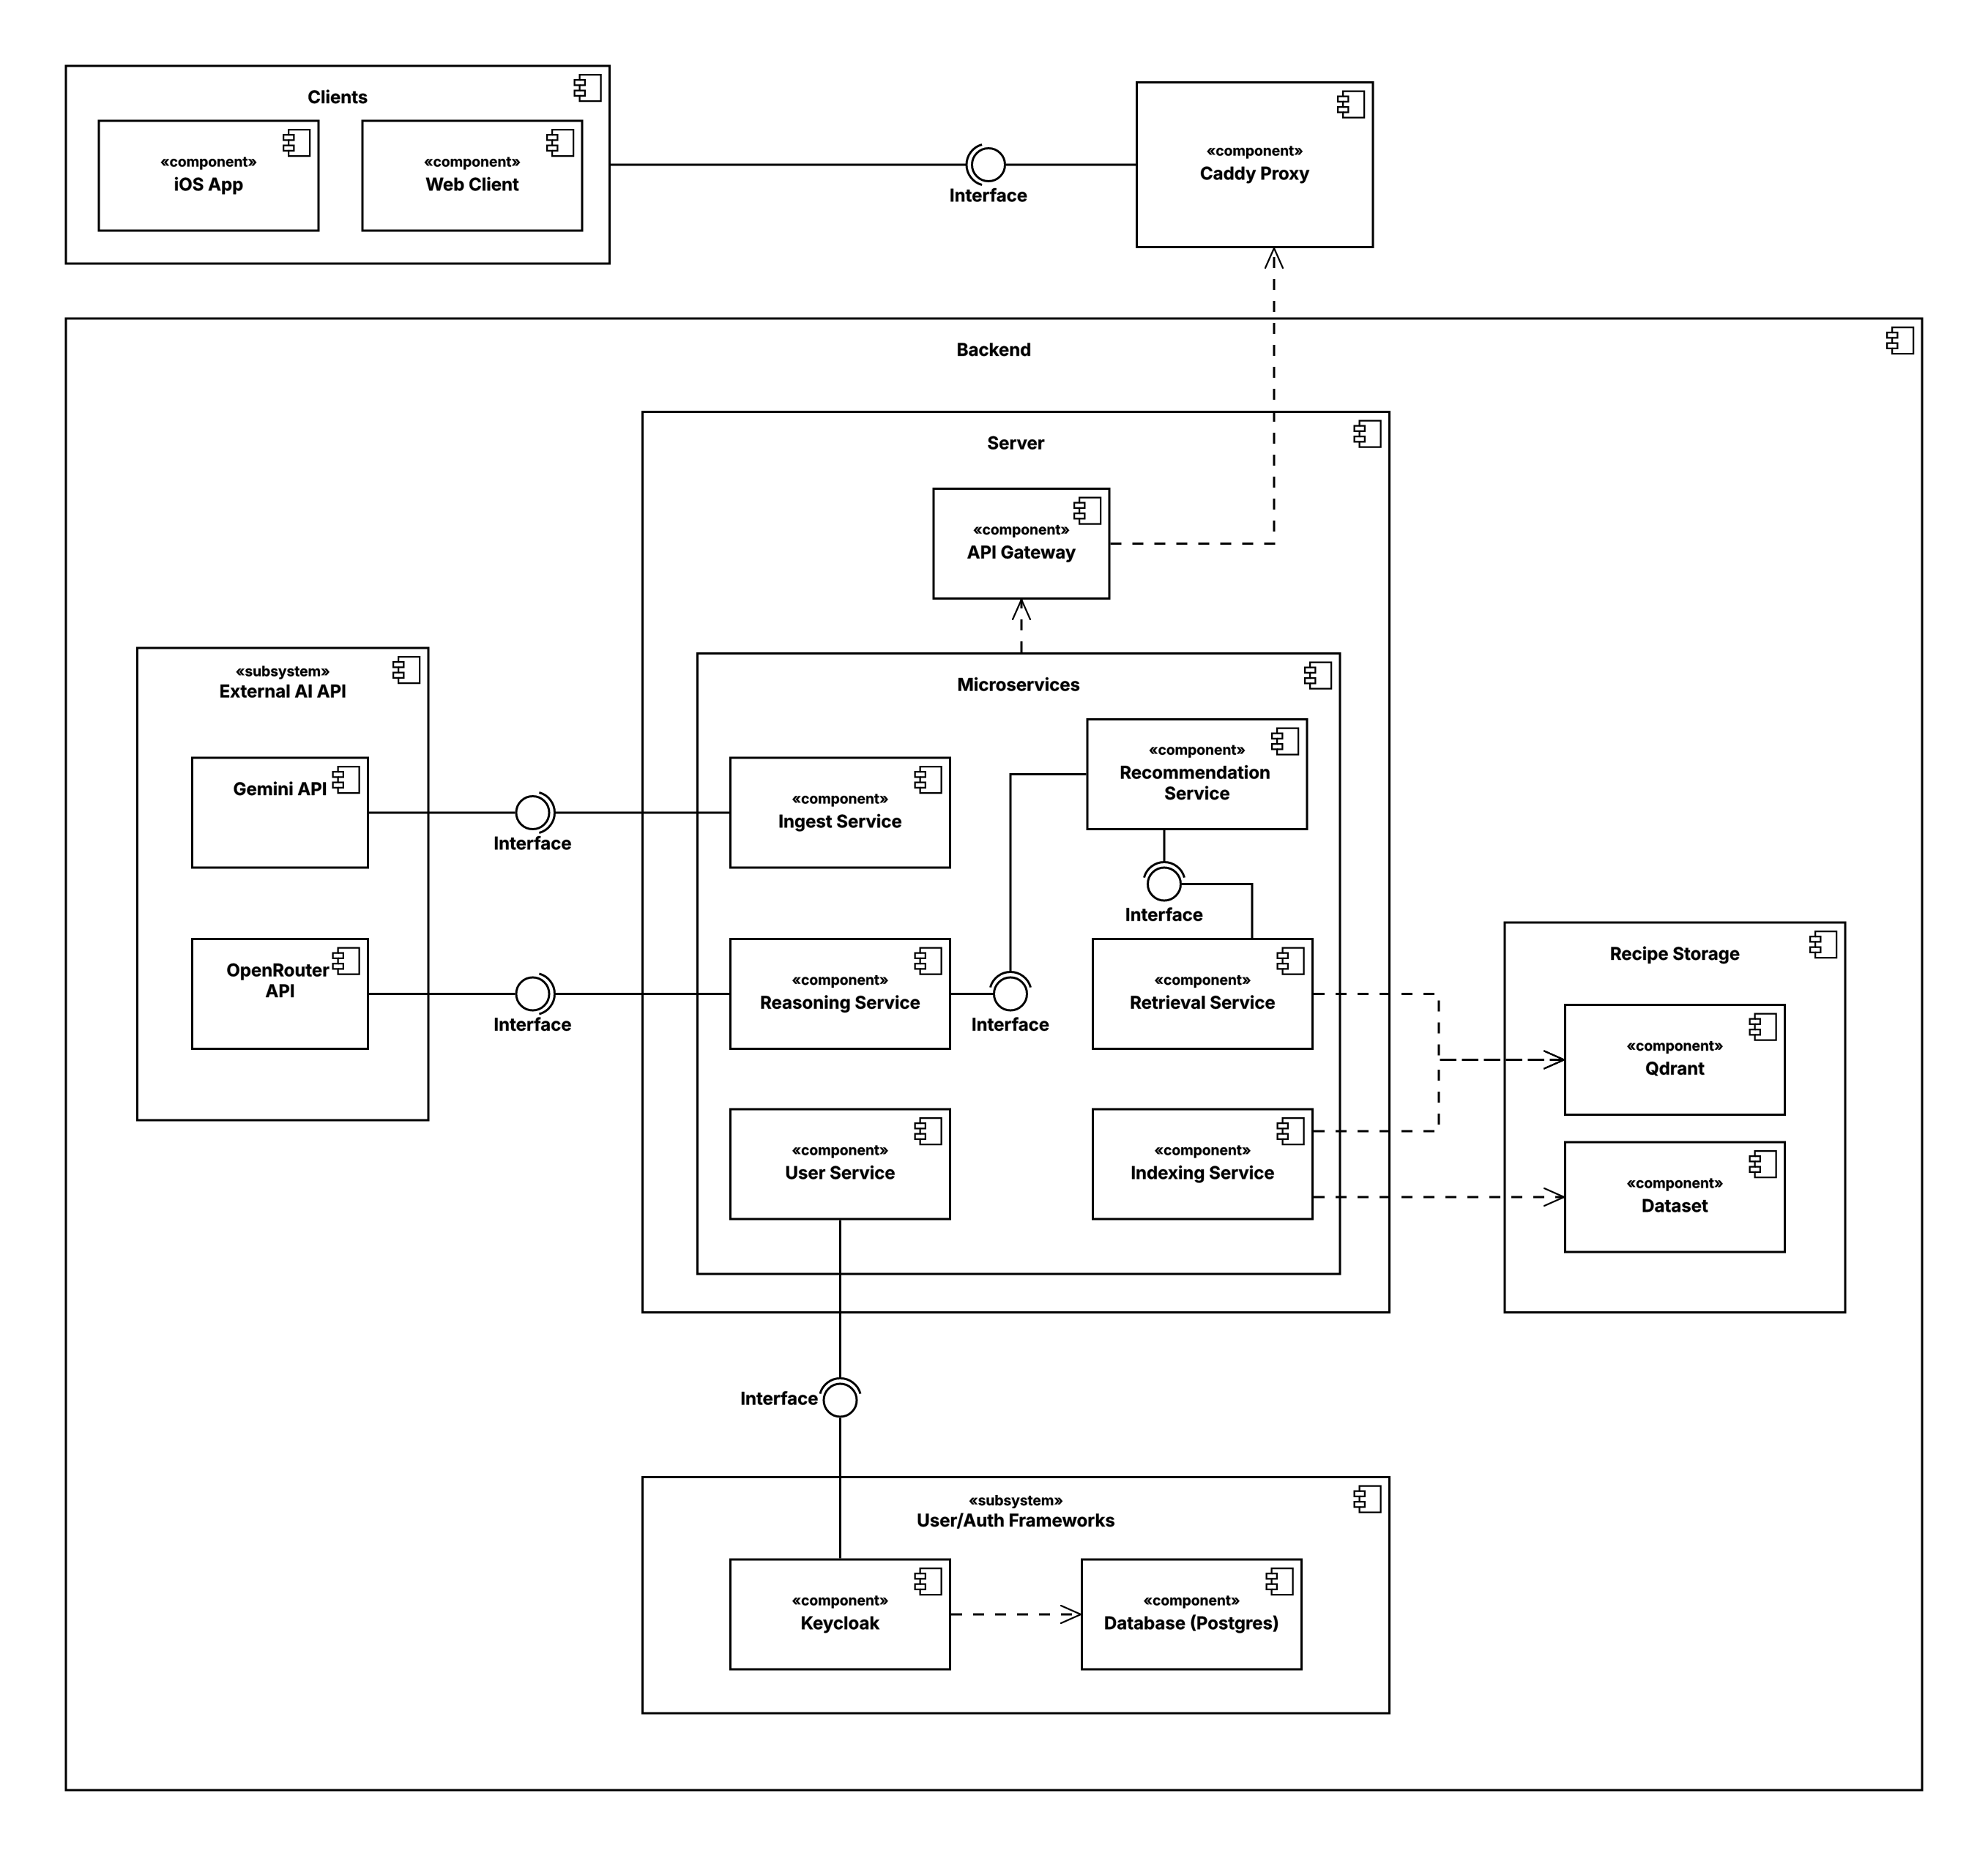
\includegraphics[width=\textwidth]{./Ressourcen/dishify_arch.png}
    \caption{Dishify system architecture and request flow.}
    \label{fig:pm-arch}
\end{figure}

\section{Method}
% TODO: Methodologies, techniques, and approaches used across the project.

\subsection{Prompt Engineering}
% TODO (REQUIRED): Prompt engineering strategies used, and how they improved the
% effectiveness of the GenAI features (reasoning explanations, recipe
% augmentation, voice/vision ingestion). Include concrete prompt patterns.

\section{Team Chart}
% TODO: Table of members, their roles, and specific contributions.
\begin{table}[!ht]
    \centering
    \caption{Team members, roles, and contributions.}
    \label{tab:pm-team}
    \begin{tabular}{@{}p{55mm}p{35mm}p{55mm}@{}}
        \toprule
        \textbf{Member} & \textbf{Role} & \textbf{Main contributions} \\
        \midrule
        Maria Chatzipavlou Arvaniti & TODO & TODO \\
        Aymen Faouel                & TODO & TODO \\
        Can Lin                     & TODO & TODO \\
        Georg Tichy                 & TODO & TODO \\
        George Trump                & TODO & TODO \\
        Chengjie Zhou               & TODO & TODO \\
        \bottomrule
    \end{tabular}
\end{table}

\section{Current Progress and Future Plans}
% TODO: Detailed status update on current progress + concrete future plans for
% project completion.

\section{Pitch Video}
% TODO: Add the link to the ~60s pitch video (also submitted as attachment).
% \url{...}

% !TeX root = ../CourseReport.tex
%=============================================================================
%  PART 3 --- USER ACCEPTANCE TESTING (UAT)
%  PAGE BUDGET: 3 pages (excluding title, ToC)          Rubric weight: 10 pts
%
%  NOTE FOR THE TEAM: the cohort composition, the seven Likert means, and the
%  free-text themes below are the figures reported in the final presentation.
%  Search for "CONFIRM" before submission.
%=============================================================================
\chapter{User Acceptance Testing}
\label{ch:uat}

\section{User Case Study: Who We Studied and Why}

Dishify's target user is the \textbf{everyday home cook who already owns food
but has no plan}: someone who cooks for themselves or a small household on most
days, shops irregularly, and repeatedly faces the same 6~p.m. question --- what
can I make with what is in the fridge right now?

We chose this profile deliberately over two alternatives. \emph{Novice cooks}
would have stressed instruction quality more than recommendation quality, and
\emph{enthusiast cooks} already own the mental index Dishify is meant to
replace, so neither would exercise the core pantry-to-recipe loop. The everyday
cook is also the group for whom our two value claims are testable: they suffer
decision fatigue, and their unused ingredients become waste.

Recruitment was therefore screened on \emph{cooking frequency} rather than
skill. Nine participants were drawn from the team's wider student and personal
network, in two deliberately different segments. \textbf{Four cook daily} ---
the group with the highest exposure to repeat decision fatigue, who would show
whether suggestions stay varied and whether a standing pantry is convenient to
maintain. \textbf{Five cook weekly} --- planning in batches from a longer-lived
pantry, who would stress ingredient coverage, tolerance for missing items, and
the usefulness of the shopping gap. Their self-reported pain points confirmed
the premise before they saw the product: \textbf{5 of 9} named ``I don't know
what to cook'' and \textbf{4 of 9} ``recipes take too long''.

The trade-off of this cohort is worth stating. It gave us participants who
genuinely have the problem and would speak candidly, but a convenience sample
is small ($n=9$), student-skewed, and prone to politeness bias --- which is why
we weight the behavioural and free-text findings at least as heavily as the
Likert means.

\section{Survey Design}

The study combined a \textbf{task-based usability test} with a
\textbf{structured survey}, so that what people did could be compared with what
they said. Participants were given the deployed web application and a short
scenario --- \emph{cook something tonight from what you actually have at
home} --- and were asked to think aloud while working through a fixed task
sequence:

\begin{enumerate}[itemsep=1pt, topsep=3pt]
    \item register an account and complete first-time setup;
    \item record any real allergies, diets, or restrictions in
          \emph{Preferences};
    \item enter a pantry reflecting their own kitchen, using typing, voice, or
          the photo scan;
    \item request recommendations and judge the ranked list;
    \item open one recipe and decide whether they would actually cook it.
\end{enumerate}

Each task carried an observed success criterion --- completed unaided, with a
hint, or abandoned --- and we noted where participants hesitated. The survey
then asked for agreement on a five-point Likert scale across seven dimensions
chosen to map onto the project's value claims rather than to generic
usability: \textbf{ease of use} and \textbf{recommendation process} (is the
pantry-first flow learnable without instruction?), \textbf{recipe relevance}
(are suggestions actually cookable from the stated pantry?),
\textbf{explanation clarity} (do ``why it fits'' and ``watch for'' carry real
information?), \textbf{allergy and diet trust} (would the user rely on the hard
filters for a restriction that matters to them?), \textbf{substitution quality}
(is the handling of missing ingredients helpful?), and \textbf{likelihood to
reuse} --- our retention proxy, and the hardest question we asked. Two
free-text questions closed the survey: what worked well, and what would have to
change before they would use Dishify again next week.

\section{Survey Execution}

All nine participants completed the full task sequence and the survey on the
deployed instance (\url{http://167.233.165.44}), each using their own real
pantry and real restrictions rather than a scripted example. Sessions ran
individually; the observer recorded task outcomes and think-aloud remarks,
after which the participant filled in the survey unobserved to limit courtesy
effects. Every participant reached a ranked result list and opened at least one
recipe, so no session was excluded, and all seven Likert dimensions received
nine responses. % CONFIRM exact session dates and observer per session.

%-----------------------------------------------------------------------------
%  TEAM ACTION (biggest single scoring gap identified in review):
%  The rubric rewards *auditable* UAT evidence. We currently report only the
%  aggregate means. If you still have the survey export, uncomment and fill the
%  table below (it fits if you shorten the "Survey Design" paragraph slightly),
%  and attach the raw CSV to the Moodle submission.
%
%  \begin{table}[!ht]
%      \centering\footnotesize
%      \caption{Per-participant task outcomes and ratings ($n=9$).}
%      \label{tab:uat-raw}
%      \begin{tabular}{@{}clccccccc@{}}
%          \toprule
%          \textbf{P} & \textbf{Cooks} & \textbf{Tasks done} & \textbf{Ease} &
%          \textbf{Proc.} & \textbf{Trust} & \textbf{Clar.} & \textbf{Rel.} &
%          \textbf{Reuse} \\
%          \midrule
%          P1 & daily  & 5/5 & 5 & 5 & 4 & 4 & 4 & 4 \\
%          ... one row per participant ...
%          \bottomrule
%      \end{tabular}
%  \end{table}
%
%  Also add: session dates, and 3--5 short anonymised verbatim quotes.
%-----------------------------------------------------------------------------

\section{Result Analysis and Evaluation}
\label{sec:uat-analysis}

\begin{figure}[!ht]
    \centering
    \begin{tikzpicture}
        \begin{axis}[
            xbar,
            width=0.74\textwidth,
            height=4.6cm,
            xmin=0, xmax=5,
            xtick={0,1,2,3,4,5},
            enlarge y limits=0.12,
            bar width=11pt,
            axis lines*=left,
            xmajorgrids, grid style={draw=black!12},
            tick align=outside,
            xlabel={mean agreement (1--5), $n=9$},
            symbolic y coords={Reuse,Substitution,Relevance,Clarity,Trust,Process,Ease},
            ytick=data,
            nodes near coords={\pgfmathprintnumber[fixed, precision=2]{\pgfplotspointmeta}},
            nodes near coords style={font=\footnotesize, anchor=west},
            every node near coord/.append style={xshift=1pt},
        ]
        \addplot[fill=dishifygreen, draw=black!40] coordinates {
            (4.67,Ease) (4.56,Process) (4.44,Trust)
        };
        \addplot[fill=dishifyorange!35, draw=black!40] coordinates {
            (4.11,Clarity) (4.00,Relevance)
        };
        \addplot[fill=dishifyorange!75, draw=black!40] coordinates {
            (3.88,Substitution) (3.67,Reuse)
        };
        \end{axis}
    \end{tikzpicture}
    \caption[User acceptance results]{Mean Likert agreement across the seven
    evaluated dimensions ($n=9$). Interaction scores (top, green) are strong;
    the content-quality and retention scores (bottom) are where the product is
    weakest.}
    \label{fig:uat-scores}
\end{figure}

Figure~\ref{fig:uat-scores} shows a clear split. Everything about
\emph{operating} Dishify scored highly --- ease of use $4.67$, recommendation
process $4.56$ --- so the pantry-first model is understood without instruction,
and our central bet on inverting the usual dish-first search was correct.
Allergy and diet trust at $4.44$ is the result we cared most about:
participants with real restrictions were willing to rely on the hard filters,
validating the decision to enforce restrictions in retrieval rather than in the
prompt.

The weaker scores concern \emph{content}, not interaction, and are consistent
with each other. Recipe relevance ($4.00$), substitution quality ($3.88$), and
likelihood to reuse ($3.67$) form a descending chain: recipes that are only
approximately cookable produce weak substitution advice, and weak substitution
advice erodes the reason to come back. Explanation clarity ($4.11$) sits
between --- the explanations are trusted, but were found terse.

The free-text answers explain the numbers. What users valued matched our value
claims almost exactly: Dishify \emph{removes the decision}, \emph{uses up food
they already own}, and the explanations \emph{make the ranking legible} rather
than arbitrary. What blocked reuse was concrete: generation felt slow;
ingredient matching was too literal (``spring onion'' not matching ``onion'');
instructions needed more detail; substitutions were weak; and onboarding did
not make the value obvious quickly enough. Participants also asked most often
for bookmarking, cooking-time and difficulty filters, health-goal filters,
recipe photos, and a print-friendly view.

\paragraph{What we incorporated, and what we did not.}
Table~\ref{tab:uat-actions} records the disposition of each finding. Two were
fixed in the time remaining; literal matching was partially addressed; latency
we measured rather than guessed, which redirected the fix from retrieval to the
explanation step; and the convenience requests are recorded as future work
rather than quietly dropped. The honest summary is that Dishify passed
acceptance on \emph{usability and trust} and did not yet pass on
\emph{retention}: a $3.67$ likelihood to reuse from a friendly cohort is a
warning, not a pass mark, and it is the number we would optimise first in any
continuation.

\begin{table}[!htbp]
    \centering
    \footnotesize
    \caption{Disposition of the main UAT findings.}
    \label{tab:uat-actions}
    \begin{tabularx}{\textwidth}{@{}p{36mm}p{22mm}X@{}}
        \toprule
        \textbf{Finding} & \textbf{Status} & \textbf{Action taken / rationale} \\
        \midrule
        Instructions too terse & Incorporated & LLM step augmentation rewrites terse directions into timed, numbered steps. \\
        Explanations too short & Incorporated & Reasoning prompt tightened to produce specific, recipe-grounded bullets. \\
        Matching too literal & Partial & Plural normalisation and token-containment matching added; synonym ontology deferred. \\
        Generation too slow & Diagnosed & Explanation is $\approx$\,47\,\% of median response time; fix is streaming/deferred explanation. \\
        Weak substitutions & Deferred & Needs an ingredient-substitution knowledge base. \\
        Onboarding, bookmarks, filters, photos, print view & Deferred & Valuable but non-core; recorded as future work (Section~\ref{sec:pm-progress}). \\
        \bottomrule
    \end{tabularx}
\end{table}

% !TeX root = ../CourseReport.tex
%=============================================================================
%  PART 4 --- GENAI SAFETY AND REFLECTION REPORT
%  PAGE BUDGET: 3 pages (excluding title, ToC)          Rubric weight: 10 pts
%
%  Required content:
%    - Safety of GenAI: safety considerations + risk-mitigation strategies
%    - Lessons learned and reflections (through the lens of your vision's
%      deliverables / KPIs / evaluations); what worked, what to improve.
%=============================================================================
\chapter{GenAI Safety and Reflection}
\label{ch:safety-reflection}

\section{Safety of GenAI}
% TODO: Safety considerations taken into account when using GenAI in Dishify and
% the strategies used to mitigate the risks. Good angles to cover:
%   - Dietary/allergy safety: restriction rules guardrails (restriction_rules.json)
%     that filter unsafe recipes before they reach the user.
%   - Prompt injection / untrusted input from voice and image ingestion.
%   - Hallucination in LLM reasoning and recipe augmentation, and how it is bounded.
%   - Privacy of user data (auth via Keycloak, what is sent to model providers).

\section{Lessons Learned and Reflections}
% TODO: Reflect through the lens of the key deliverables / KPIs / evaluations from
% the project vision. What worked well, what could be improved in future projects,
% and how this project shaped your understanding of GenAI and its applications.

% !TeX root = ../CourseReport.tex
%=============================================================================
%  NOVELTY / VALUE PROPOSITION
%  PAGE BUDGET: keep it short (~1 page)                 Rubric weight: 5 pts
%
%  Scoring notes from the criteria:
%    - Simple wrappers of GenAI APIs will NOT gain points.
%    - No clones of existing services.
%    - Must introduce a new approach, workflow, or combination of methods
%      compared to the industry baseline.
%=============================================================================
\chapter{Novelty and Value Proposition}
\label{ch:novelty}

Dishify addresses a common everyday problem: deciding what to cook with the ingredients already available at home. The value of the system is that it reduces the effort of searching manually through recipe websites or asking a general chatbot for ideas. Instead, the user can enter available ingredients, dietary restrictions, or allergies, and receives recipe recommendations that include matched ingredients, missing ingredients, and an explanation of why each recipe fits the situation.



The novelty of Dishify is that it is not a thin wrapper around a GenAI API. A simple GenAI wrapper would send the full user request directly to a language model and return a generated answer. Dishify follows a more controlled pipeline. First, recipes are retrieved from a structured recipe dataset using vector search. Then, the results are ranked based on how well they match the user's available pantry ingredients. This makes the recommendation process more deterministic and transparent than a pure chatbot-based approach.



Another important part of the value proposition is how dietary restrictions and allergies are handled. Instead of relying only on the language model to remember these constraints, Dishify treats them as explicit user preferences and uses them as guardrails in the recommendation process. This helps reduce unsuitable recommendations and increases user trust, especially for users who need to avoid specific ingredients.



Dishify also combines multiple input methods into one workflow. Users can type ingredients manually, but the system can also support voice and image input through the ingest service. Detected ingredients from speech or images are then passed into the same recommendation pipeline. This creates a more convenient user experience, because the user does not need to formulate a perfect prompt manually.



Compared to the industry baseline, Dishify is neither only a recipe search engine nor only a chatbot. Traditional recipe platforms mainly rely on keyword search and manual filters, while general chatbots can generate recipes but usually do not use a curated recipe database, pantry-based ranking, and structured user restrictions together. Dishify combines these methods into one hybrid system: vector retrieval provides relevant recipe candidates, inventory-aware ranking personalizes the results, restriction guardrails improve safety, and GenAI is used to explain and enhance the recommendations. This combination creates a more practical, transparent, and user-centered cooking assistant.
% !TeX root = ../CourseReport.tex
%=============================================================================
%  ACKNOWLEDGMENT OF GENAI USAGE
%=============================================================================
\chapter{Acknowledgment of GenAI Usage}
\label{ch:genai-usage}

Generative AI was used as an assistant in the product, during development, and
while preparing this report. The team reviewed and checked AI-assisted outputs
before relying on them.

\section{In the Product}

Generative AI supports Dishify's multi-modal input and recipe assistance
features. Its outputs are constrained by the application flow and checked before
they are shown or used.

\section{During Development}

The team used AI coding assistants for implementation support, debugging, and
documentation tasks. AI-assisted changes were reviewed by team members and
validated through the same testing and review process as other work.

\section{In This Report}

This document was drafted and revised with assistance from large language
models. The final content was checked against the repository, the deployed
system, and the team's own evaluation results.

\noindent
\textbf{User data was not generated.} The acceptance-testing numbers are the
team's own survey results and were not inferred or fabricated. The team reviewed
and edited the report before submission.


%=============================================================================
%  BIBLIOGRAPHY
%=============================================================================
\printbibliography[heading=bibintoc, title=References]

\end{document}
